\documentclass[a4paper, 12pt]{article}
\usepackage{subfiles}

% PACKAGES
%% document formatting
\usepackage[default]{sourcesanspro}
\usepackage[nottoc,numbib]{tocbibind}

%% languages
\usepackage[ngerman]{babel}
\usepackage{csquotes}

%% hyperlinks
\usepackage{hyperref}
\usepackage{url}

%% graphics
\usepackage{graphicx}
\usepackage{geometry}

%% citation
\usepackage{acronym}
\usepackage[style=ieee]{biblatex}
\usepackage{floatrow}

%% code listings
\usepackage{listings}
\usepackage{xcolor}


% CONFIGURATION
\setlength{\parindent}{0pt}
\hfuzz=10pt 

%% sources
\addbibresource{sources.bib}

%% document link format
\hypersetup{
  colorlinks   = true, %Colours links instead of ugly boxes
  urlcolor     = blue, %Colour for external hyperlinks
  linkcolor    = blue, %Colour of internal links
  citecolor   = red %Colour of citations
}

%% list of figures
\renewcommand{\listoffigures}{\begingroup
\tocsection
\tocfile{\listfigurename}{lof}
\endgroup}

%% listing style
\definecolor{codegreen}{rgb}{0,0.6,0}
\definecolor{codegray}{rgb}{0.5,0.5,0.5}
\definecolor{codepurple}{rgb}{0.58,0,0.82}
\definecolor{backcolour}{rgb}{0.95,0.95,0.92}

\lstdefinestyle{mystyle}{
    backgroundcolor=\color{backcolour},   
    commentstyle=\color{codegreen},
    keywordstyle=\color{magenta},
    numberstyle=\tiny\color{codegray},
    stringstyle=\color{codepurple},
    basicstyle=\ttfamily\footnotesize,
    breakatwhitespace=false,         
    breaklines=true,                 
    captionpos=b,                    
    keepspaces=true,                 
    numbers=left,                    
    numbersep=5pt,                  
    showspaces=false,                
    showstringspaces=false,
    showtabs=false,                  
    tabsize=2
}

\lstset{style=mystyle}

\begin{document}
    \begin{titlepage}
    
\includegraphics[width=0.4\textwidth]{images/HFT_logo}
    \centering
    \vspace{1.5cm}
    {\par \LARGE Erarbeitung und Evaluation einer Laborumgebung zum Thema Webapplication Firewall\par}
    \vspace{1cm}
    {\par \large Bachelor Thesis\par}
    {\par \large im Studiengang Informatik\par}
    \vfill
    \begin{table}[!hbt]
        \centering
        \begin{tabular}{ll}
            Betreuender Dozent:         & Prof. Dr. Jan Seedorf           \\
            Betreuer des Unternehmens:  & Oliver Paukstadt                \\
            Vorgelegt am:               & \today                          \\
            Vorgelegt von:              & Lukas Reinke (Mat. NR. 1001213)
        \end{tabular}\label{tab:info}
    \end{table}
\end{titlepage}
    \subsection*{Eidesstattliche Erklärung}
Hiermit erkläre ich, dass ich die vorliegende Abschlussarbeit selbständig verfasst und keine anderen als die angegeben Quellen und Hilfsmittel verwendet habe.
Alle Stellen, die wörtlich oder sinngemäß aus den Quellen entnommen wurden, sind als solche kenntlich gemacht.
Weiterhin erkläre ich, die die Arbeit nicht anderweitig veröffentlicht oder an anderer Stelle als Prüfungsleistung vorgelegt wurde.

\vspace{50px}

\begin{tabular}{@{}p{2.5in}p{2.5in}@{}}
  \dotfill & \dotfill \\
  Ort, Datum & Lukas Reinke \\[5\bigskipamount]
\end{tabular}

\pagebreak
    \section{Abstract}
Hier könnte ihr abstract stehen.

\pagebreak
    \tableofcontents
\pagebreak

\section{Abkürzungsverzeichnis}

\begin{acronym}
    \acro{dmz}[DMZ]{Demilitarisierten Zone}
    \acro{dsgvo}[DSGVO]{Datenschutz-Grundverordnung}
    \acro{http}[HTTP]{Hypertext Transfer Protocol}
    \acro{https}[HTTPS]{Hypertext Transfer Protocol Secure}
    \acro{itsig}[IT-SiG]{IT-Sicherheitsgesetzes}
    \acro{mim}[MITM]{Man-in-the-middle}
    \acro{nat}[NAT]{Network Adress Translation}
    \acro{tls}[TLS]{Transport Layer Security}
    \acro{url}[URL]{Uniefied Resource Locator}
    \acro{rfc}[RFC]{Request for Comments}
    \acrodefplural{rfc}[RFCs]{Requests for Comments}
    \acro{vm}[VM]{Virtuelle Maschine}
    \acrodefplural{vm}[VMs]{Virtuelle Maschinen}
    \acro{waf}[WAF]{Web Application Firewall}
    \acrodefplural{waf}[WAFs]{Web Application Firewalls}
    \acro{xss}[XSS]{Cross Site Scripting}
\end{acronym}

\pagebreak

\listoffigures

\pagebreak

    %chapters
    \section{Einleitung}
    \label{sec:introuduction}

% WAF relevant weil:
%   markt wachstum
%   DSGVO implizit relevant

Das Feld der \ac{waf} gewinnt aktuell immer mehr an Relevanz.
Dem Markt wird in den nächsten fünf Jahren ein jährliches Wachstum um 19,9 \% auf 14,6 Mrd.\$ vorhergesagt \cite{WebApplicationFirewall}.
Auch Ausarbeitungen zum \textit{Stand der Technik} wie sie zum Beispiel im Deutschen \ac{itsig} und der \ac{dsgvo} gefordert werden, beschreiben eine \ac{waf} als notwendig zur Absicherung einer Webanwendung\cite[3.1.19 Schutz von Webanwendungen]{StandTechnik}.

% was soll vermitttelt werden?
%   was mach WAF
%   wie nutzt man WAF
%   wie greift man WAF an

Diese Bachelor Thesis beschäftigt sich mit der Erarbeitung von Lerneinheiten und einer Laborumgebung anhand derer das Thema \ac{waf} vermittelt werden kann.
Es werden Design beziehungsweise Implementierung einer \ac{waf} betrachtet.
Auch werden Themen vermittelt, die für den Betrieb einer \ac{waf} in einem produktiven Umfeld relevant sind.
Dazu zählen zum Beispiel Deployment und Anpassung einer \ac{waf} an die zu schützende Webanwendung.

%% TODO

\pagebreak
    %\subsection{Umfang und Abgrenzung}
    %\input{./chapters/01.2_Umfang.tex}
    %\pagebreak

    \section{Theoretische Grundlagen}
    \label{sec:theoretical-foundations}
    \subsection{Hypertext Transfer Protocol}
    Das \ac{http} ist ein Protokoll, das in der Internet-Kommunikation zum Einsatz kommt.
Es dient zur Übertragung von Daten zwischen einem Client und einem Server und wird hauptsächlich zur Auslieferung beziehungsweise Bedienung von Webanwendungen genutzt.
Seit der Einführung im Jahr 1991 wurde es in mehreren \acp{rfc} erweitert und ist inzwischen in Version drei\cite{onlineIETFErhebtHTTP2022}.\\

Das der \ac{http}-Kommunikation zu Grunde liegende Interaktionsmuster erfolgt nach den \textit{Request-Response-Pattern}.
Ein Client beginnt die Kommunikation und fragt Daten oder Daten-Operationen an einem Server an.
Der Server beantwortet diese Anfrage\footnote{Im folgenden werden \ac{http}-Anfrage und das Englische \ac{http}-Request synonym verwendet. Das Gleiche gilt für \ac{http}-Antwort und \ac{http}-Response} und sendet dem Client Informationen wie die Verarbeitung erfolgt ist und die Angeforderten Daten.
Diese Kommunikation erfolgt über TCP.

Ist ein Request-Response Cycle abgeschlossen, wird die TCP-Verbindung gekappt und der Server kann keine weiteren Nachrichten an den Client schicken bis dieser eine neue Anfrage startet.
Übertragen werden können Texte in diversen Formatierungen wie beispielsweise \textit{HTML-Dokument} oder \textit{JSON-Strings}, es ist jedoch auch möglich binäre Daten wie \textit{Bilddateien} zu übertragen.
HTML ist ein \textit{Plaintext}-Protokoll, die Kommunikation erfolgt unverschlüsselt.
Außerdem ist \ac{http} textbasiert, eine Nachricht wird in Textform übertragen und ist menschenlesbar.

Die oben beschriebenen Eigenschaften beziehen sich auf \ac{http} in Version 1.
Seit dieser Version wurden einige Erweiterungen an \ac{http} vorgenommen, hauptsächlich mit dem Ziel die Kommunikationsgeschwindigkeit des Protokolls zu erhöhen.
So kann TCP-Pipelining genutzt werden um mehrere TCP-Nachrichten nacheinander zu schicken ohne Bestätigung des Erhaltens der Nachricht abwarten zu müssen.
Außerdem werden Push-Nachrichten unterstützt:
Der Server kann durch Aufrechterhaltung einer TCP-Verbindung weitere \ac{http}-Nachrichten an den Client schicken.
Mit Version 3 wurde \ac{http} außerdem auf das Stream-basierte QUIC Protokoll umgestellt um die Kommunikation weiter zu optimieren\cite{OverviewHTTPHTTP2023}.\\

Da die grundlegende Funktion von \ac{http} 1.0 und 1.1 ausreichend ist, um eine \ac{waf} zu erklären, wird im Folgenden nur diese betrachtet.

\paragraph{\ac{http}-Nachrichten \cite{HTTPMessagesHTTP2024}}
\ \\
Die grundlegende Einheit einer \ac{http}-Kommunikation wird als \textit{Nachricht} bezeichnet.
Da \ac{http} ein Klartext-Protokoll ist, werden diese in menschenlesbarer Form als Text übertragen.
Eine Nachricht besteht aus einer \textit{Start-Zeile}, die die Nachricht entweder als Anfrage oder Antwort identifiziert.
In den beiden Fälle ist der Aufbau dieser Zeile unterschiedlich:

\begin{figure}[!hbt]
     \centering
     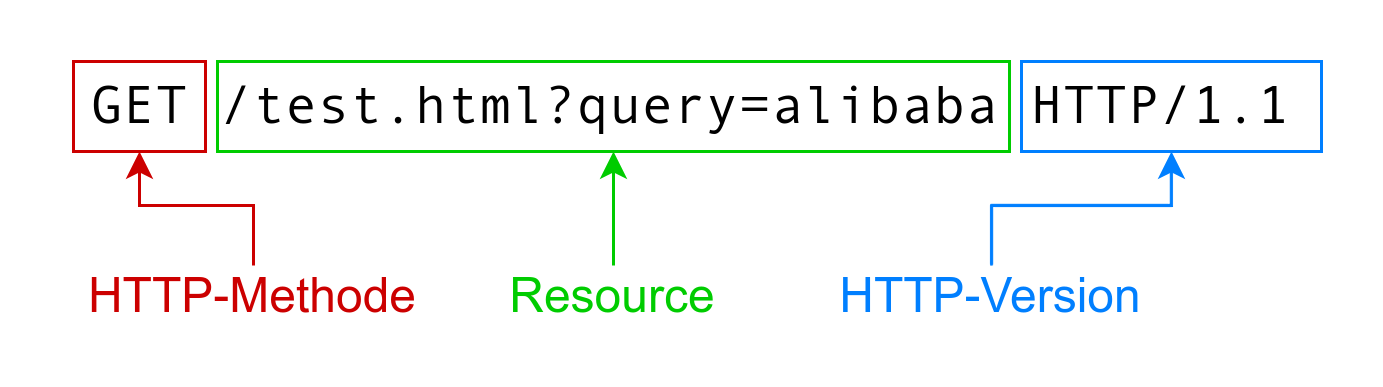
\includegraphics[width=0.9\textwidth]{./images/HTTP-Requestline.png}
     \caption{Beispiel für eine \ac{http} Request-Zeile}
     \floatfoot{Quelle: Eigene Darstellung}
     \label{fig:http-requestline}
 \end{figure}

\begin{description}
     \item[Request-Zeile:] Ein \ac{http}-Request ist durch eine \textit{Request-Zeile} identifiziert. Diese ist in drei Teile aufgeteilt (siehe Abbildung \ref{fig:http-requestline}).
     \begin{description}
          \item[Die \ac{http}-Methode] beschreibt die Operation, die der Server ausführen soll.
          Die Operationsbezeichner können auch \textit{\ac{http}-Verben} und \textit{\ac{http}-Nomen} genannt werden.
          Syntaktisch basieren die Methoden auf dem FTP Protokoll, das älter ist und mit Operationen wie GET und PUT arbeitet.
          In höheren Versionen wird der Satz an Verben und Nomen jedoch um weitere Methoden, wie zum Beispiel PATCH oder OPTIONS, erweitert.
          \item[Die Resource] beschreibt das angefragte Objekt, üblicherweise in einer \ac{url}. 
          Optional kann die angefragte Resource mit einem Fragezeichen gefolgt von einem sogenannten \textit{Query String} noch spezifiziert beziehungsweise gefiltert werden.
          \item[Die \ac{http} Version] die angibt in welcher Version die folgende Nachricht verfasst ist. 
     \end{description}
\end{description}

\begin{figure}[!hbt]
     \centering
     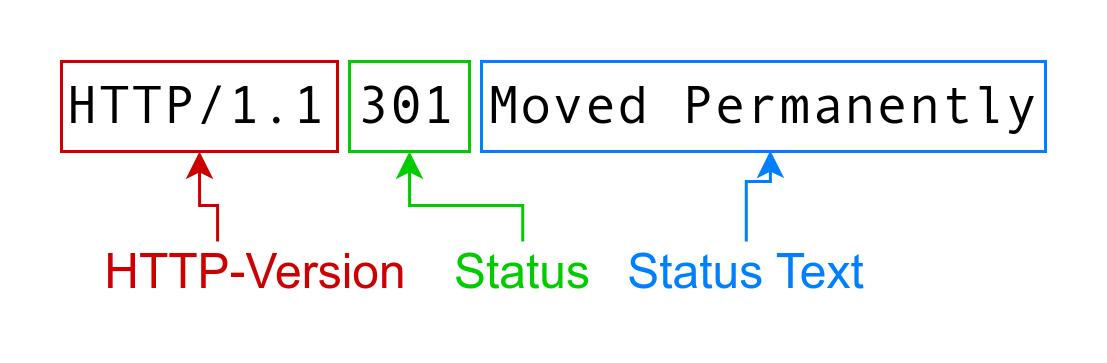
\includegraphics[width=0.9\textwidth]{./images/HTTP-Statusline.png}
     \caption{Beispiel für eine \ac{http} Status-Zeile}
     \floatfoot{Quelle: Eigene Darstellung}
     \label{fig:http-statusline}
 \end{figure}


\begin{description}
     \item[Status-Zeile:] Die Antwort auf einen Request beginnt mit einer Status-Zeile in einem eigenen Format, die wie die Request-Zeile aus drei Teilen besteht (siehe Abb. \ref{fig:http-statusline}).
     \begin{description}
          \item[Die \ac{http} Version] gibt, wie an dritter Stelle des \ac{http}-Requests, die \ac{http}-Version der folgenden Nachricht an.
          \item[Der Status Code] ist ein dreistelliger Zifferncode, der eine Rückmeldung über die Verarbeitung des Request gibt. 
          Die erste Stelle signalisiert um welche Art des Ereignisses es sich handelt.
          So stehen zum Beispiel die Codes 2xx für eine erfolgreiche Verarbeitung, während 4xx auf einen Fehler auf Client-Seite hindeutet.
          Die zwei folgenden Stellen geben genauer Aufschluss wie der Status ist\cite{HTTPResponseStatus2023}.
          \item[Der Status Text] ist ein beliebiger Text, der den Status genauer beschreibt.
          Im \ac{http} Standard ist zwar nicht vorgeschrieben wie der Text auszusehen hat, es gibt jedoch Konventionen\cite{HTTPResponseStatus2023}.
     \end{description}
\end{description}

Nach der Start-Zeile folgen sowohl in einem \ac{http}-Request als auch in der Response zwei weitere Abschnitte. 
Diese werden genutzt, um der Nachricht weitere Informationen hinzuzufügen.

Die \textbf{\ac{http}-Header} sind Key-Value Paare. 
Der Key ist ein Schlüsselwort, dass unter Berücksichtigung der Groß-Kleinschreibung ausgewertet wird. 
Der zugehörige Wert (Value) geht bis zum Zeilenende und darf darum keinen Zeilenumbruch enthalten, da dadurch der Beginn des nächsten Key-Value-Paares angezeigt wird.
Die Header teilen sich in Unterkategorien wie beispielsweise \textit{Request-} oder \textit{General-Header} auf; an dieser Stelle ist es im Rahmen dieser Thesis jedoch nicht notwendig, weiter in die Tiefe zu gehen.
Eine relevante Header-Gruppe sind die \textit{Representation-Header}, die die Formatierung des \ac{http}-Bodies genauer spezifizieren.
Hier kann der Datentyp und die Formatierung des Bodies angegeben werden.
Es is beispielsweise möglich zwischen einem Text und einem JSON-Objekt zu unterscheiden.

Der \textbf{\ac{http}-Body} enthält die Daten die mit der \ac{http}-Nachricht versendet werden und ist optional.
Im Body können sich beliebige Daten befinden: base64 codierte Daten, Datenstrukturen im JSON-Format oder einfacher Text als ASCII oder UTF-8 encodiert.\cite{HTTPMessagesHTTP2024}.\\

Wie oben beschrieben, bietet \ac{http} zahlreiche Möglichkeiten an, einem Server Daten zu übergeben oder von einem solchen Daten zu erhalten.
Alle Felder werden verarbeitet und bieten somit theoretisch die Möglichkeit zur Übermittlung schadhafter Daten.
Auch die Möglichkeit zur codierten Übertragung, speziell im \textit{\ac{http}-Body}, kann zu diversen Angriffsvektoren führen.
Eine \ac{waf} muss in der Lage sein, alle dieser Parameter überblicken zu können um effektiven Schutz zu bieten.

\pagebreak    
    \subsection{Verschlüsselung}
    \input{chapters/02.2_Verschlüsselung.tex}
    \subsection{Weiterleitung von Netzwerkkommunikation}
    In den meisten Fällen ist es nicht ohne Weiteres möglich eine direkte Verbindung zwischen einem Client und einem Server aufzubauen.
Die Gesamtzahl aller IPv4 Adressen ($2^{32}$) reicht inzwischen nicht mehr aus um allen Geräten, die eine Internet Verbindung besitzen, eine eigene, öffentliche IP-Adresse zuzuordnen.
Auch ist es zum Teil notwendig Netzwerkverkehr zu einem Server umzuleiten.
Beispielsweise wenn auf einem Server mehrere Services betrieben werden, die unter unterschiedlichen Namen erreichbar sein sollen,
Auch Sicherheitsbedenken können es notwendig machen eine interne Netzstruktur für einen externen Beobachter ersichtlich zu machen.

Aus den oben genannten Gründen muss in einigen Fällen der Netzwerkverkehr weitergeleitet beziehungsweise umgeschrieben werden.
Auch eine \ac{waf} operiert auf Basis einer solchen Technologie.
Zwei dieser Technologien werden im Folgenden genauer beschrieben.\\

\textbf{\ac{nat}} ist ein Oberbegriff für Technologien mit Hilfe derer es möglich ist auf Ebene der Schicht 2 des TCP/IP Modells Netzwerkverkehr zu verändern.
Das heißt, Traffic kann durch umschreiben der IP-Adresse in einem Paket an einem Relay-Punkt an unterschiedliche Netzwerk-Teilnehmer weitergeleitet werden.
Ein Einsatzgebiet für \ac{nat} ist zum Beispiel wenn mehrere Netzwerk-Teilnehmer mit einer IP-Adresse auf das Internet zugreifen.

Aus Sicht der Netzwerksicherheit bietet \ac{nat} Vorteile.
Da auf einer niedrigen TCP/IP Schicht operiert wird, kann keine Transportverschlüsselung geöffnet werden und Inhalte betrachtet werden.
Protokolle die Verschlüsselung anbieten arbeiten auf höheren Schichten.
Der einzige kleine Vorteil kann die Verschleierung einer Internen Netzwerkstruktur sein\cite{NATNetworkAddress}.\\

Auf der Anwendungsschicht (Layer 4) operieren \textbf{Netzwerk Proxys}.
Diese können TCP/IP Layer 4 Protokolle auf Basis von Informationen in den Nachrichten weiterleiten.
Anstatt eine Verbindung direkt mit dem Ziel aufzubauen kommuniziert ein Client mit dem Proxy, der dann mit dem gewünschten Server kommuniziert.
Ein Proxy dient also als Vermittler zwischen Client und Server.
Für das Thema \ac{waf} speziell relevant sind \textbf{Reverse Proxies}.
Ein Reverse Proxy befindet sich in einem privaten Netzwerk mit dem Ziel-Server, ist aber als einziger in diesem Netzwerk auch in der Lage mit einem öffentlichen Netz zu kommunizieren(Siehe Abbildung \ref{fig:revprox}).
Eingehender Netzwerkverkehr wird Beispielsweise anhand der \ac{url} in einem HTTP-Paket an den zugeordneten Server weitergeleitet.
Der Proxy hält die Verbindung zu einem Client aktiv bis er eine Antwort vom Server erhält.
Antwortet dieser ordnet der Reverse Proxy diese dem passenden Client zu, gibt die Antwort des Servers weiter und schließt die Verbindung zum Client.
Transportverschlüsselung wird von dem Reverse Proxy vorgenommen.

\begin{figure}[!hbt]
    \centering
    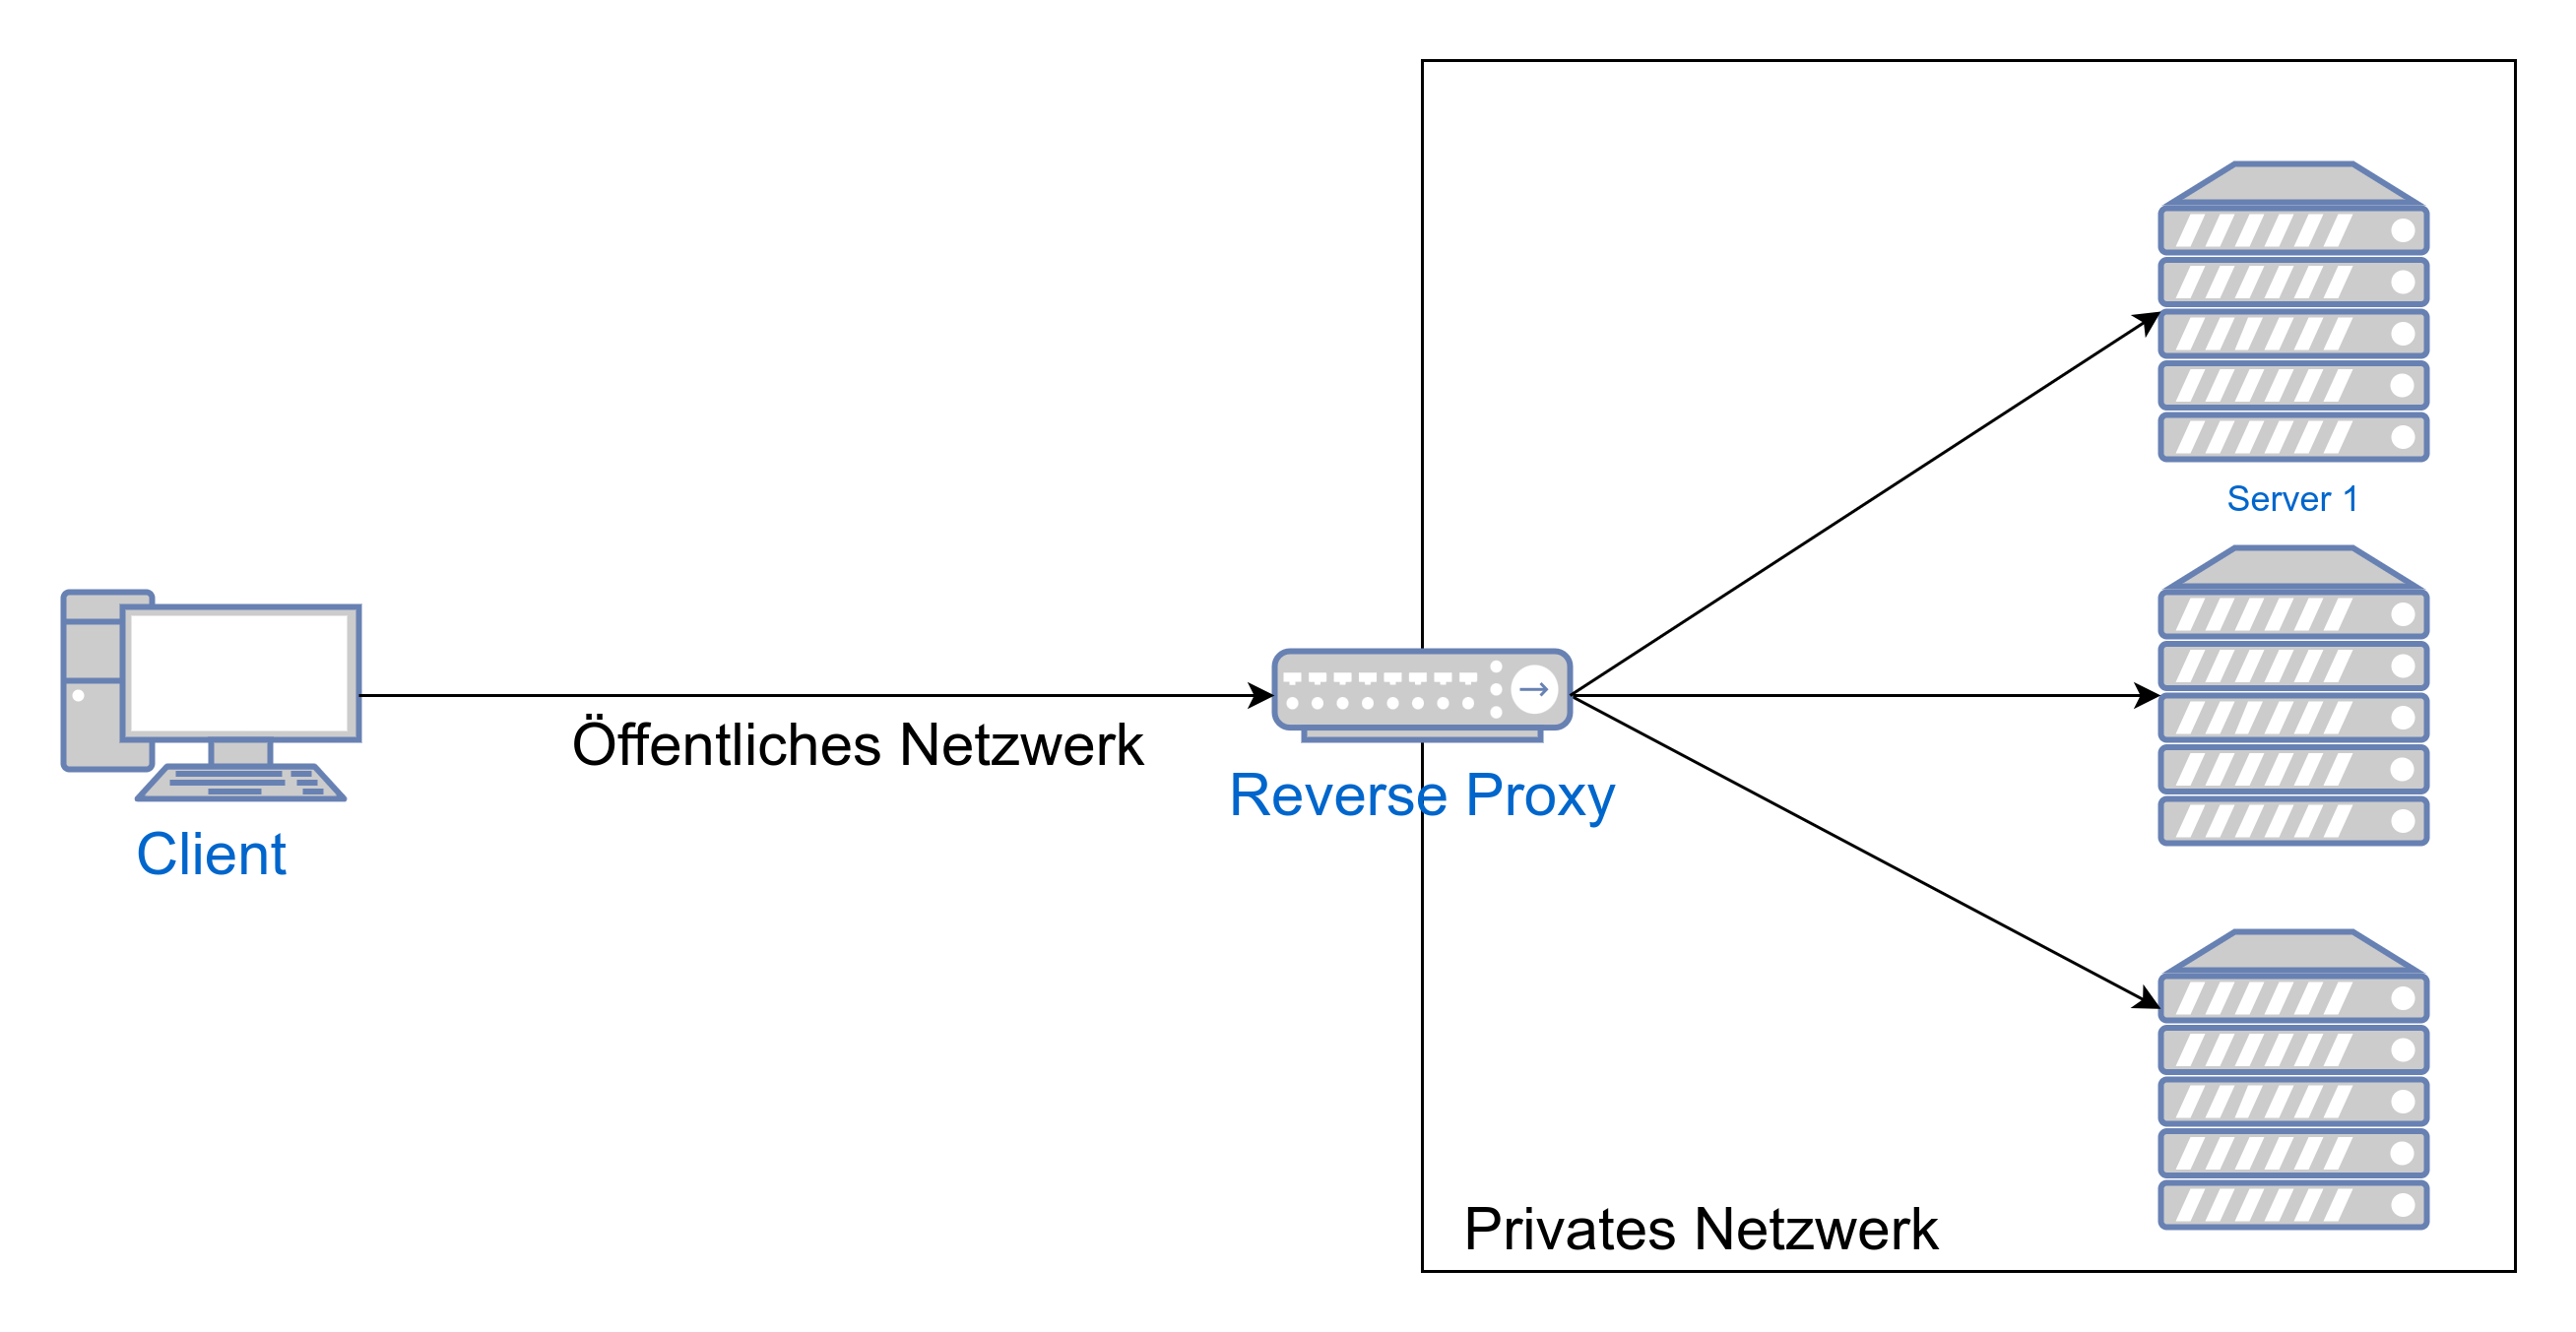
\includegraphics[width=0.9\textwidth]{./images/reverse-Proxy.png}
    \caption{Schematische Darstellung eines Reverse Proxies}
    \label{fig:revprox}
\end{figure}

Hieraus ergeben sich einige positive Sicherheitsaspekte.
Da einem Reverse Proxy Kommunikation unverschlüsselt vorliegt kann diese Inspiziert werden.
Anwendungen die Netzwerksicherheit auf Layer 4 betreiben operieren als Reverse Proxy um tief in Netzwerkverkehr blicken zu können.
Eine \ac{waf} kann konzeptionell als Modul auf einem Reverse Proxy betrachtet werden\cite{WasIstReverse}.

\pagebreak
    %\subsection{OWASP Top-Ten}
    %% Standard für die Sicherheit von Webanwendungen 
% wichtigsten Sicherheitsrisiken für Webanwendungen
% Regelmäßig upgedatet um den gegenwärtigen stand darzustellen
% 
% - Broken Access Control
%     - Fehler die zu unerlaubten Privilegien führe
%     - Least-privilege Prinzip
%     - Privilege escalation
% - Verschlüsselungsfehler
%     - veraltete Protokolle
%     - neue Schwachstellen
% - Injection
%     - SQL, noSQL, LDAP, ...
% -  unsicheres Design
%     - Der Applikation inherente Fehler
% - Fehlkonfigurationen
% - Anfällige und veraltete Komponenten
% - Identifizierung- und Authentifizierungsfehler
%     - Fehler in Zugangskontrolle
% -  Fehler bei der Software- und Datenintegrität
%     - Fehler bei der Prüfung von Daten-Validität(Updates, Externe Pakete,...)
% - Fehler beim Logging
% - Server-Side Request Forgery


\pagebreak
    \subsection{Web Application Firewall}
    % - Sicherheits-Applikation/ Spezielle Firewall
%    - Gefordert in diversen Compliance Richtlinien
% - was mach eine WAF im Prinzip?
%     - Zwischen Client und Server
%     - Analysiert Datenverkehr
% - Fokus auf web-Protokolle
%     - auf TCP/IP Layer 5
%     - HTTP, HTTPS, FTP
% - Traffic Analyse in Tiefe (Request & Response)
%     - HTTP (kapitel 5.2) beschreibt diverse Angriffswege
%     - Erkennung anhand von Regeln
%         - Black- vs. whitelisting
%         - Vordefiniertes Regelwerk
\label{chap:waf-theory}
Ein \ac{waf} ist eine Sicherheits-Applikation, die in der Lage ist den Datenverkehr zu und von einer Web-Anwendung zu Analysieren.
Hierbei werden die Übertragenen Inhalte in der Tiefe auf schädliche Inhalte überprüft.
Der in Abbildung \ref{fig:waf-porcess-flow} dargestellte Prozessablauf beschreibt wie eine \ac{waf} mit eingehenden Nachrichten umgeht.

\begin{figure}[!hbt]
    \centering
    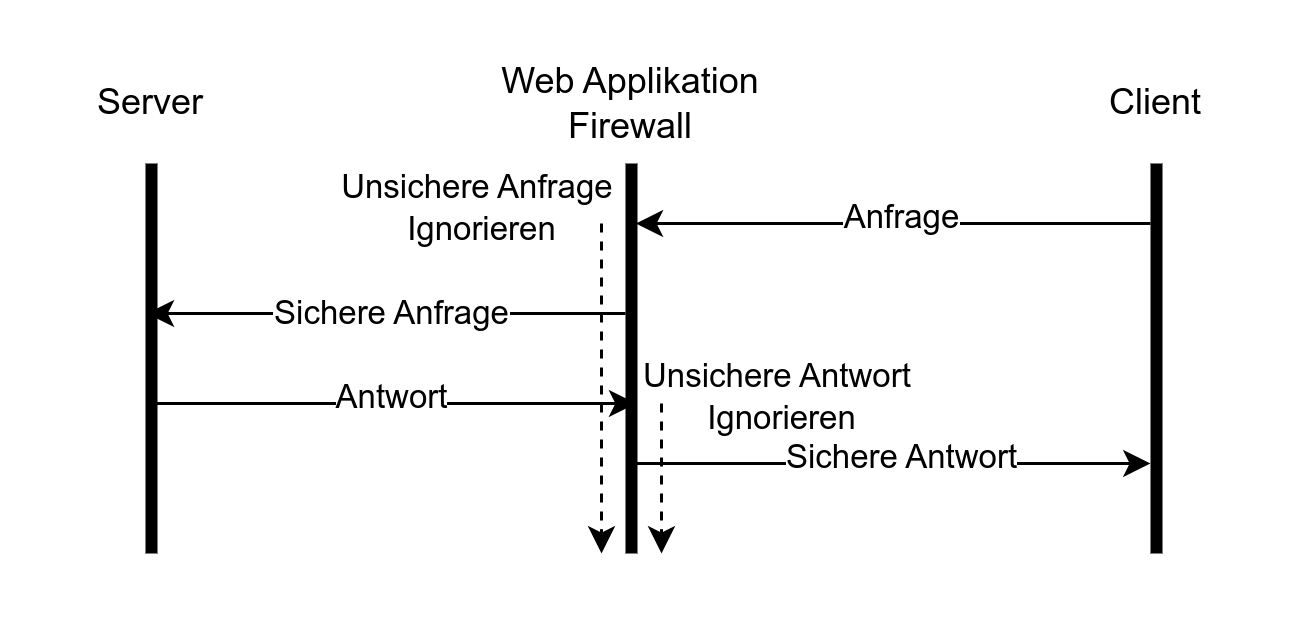
\includegraphics[width=0.9\textwidth]{./images/Waf-Process-fliow.png}
    \caption{Prozess Ablauf der Verarbeitung durch eine \ac{waf}}
    \label{fig:waf-porcess-flow}
\end{figure}

Das grundlegende Muster ist, dass einen Nachricht an der \ac{waf} eintrifft und von dieser an den Server weitergegeben wird.
Dieser Verarbeitete die Anfrage und sendet seine Antwort an die \ac{waf} die die Antwort an den Client weiterleitet.
Der Server kennt in diesem Muster den CLient nicht.
Die \ac{waf} ordnet der Anfrage die zugehörige Antwort zu.
Als schädlich erkannte Inhalte können sowohl in einer Anfrage als auch Antwort abgelehnt werden.
Anstatt einer abgelehnten Nachricht kann eine \ac{waf} auch eine eigene Antwort an den Client senden.
Das ermöglicht Nutzer festzustellen, dass ein Fehler in seiner Anfrage oder der Konfiguration der \ac{waf} vorliegt.
Mittels einer ID, die der ersetzten Antwort angehängt wird lässt sich das Verhalten im Nachhinein nachvollziehen
Neben den beiden Möglichkeiten weiterleiten und Ablehnen kann eine \ac{waf} die in einer Anfrage erkannten schädlichen Inhalte auch neutralisieren und die Nachricht weitergeben.

Eine \ac{waf} wird in produktiven Umgebungen in einem Netzwerk \textit{vor} den zu schützenden Anwendungen positioniert.
Das heißt der geschützte Server befindet sich in einer \ac{dmz}.
Eine \ac{dmz} ist ein, von anderen Netzwerkaktivitäten abgeschnittenes Netzwerksegment, das nur durch die \ac{waf} sowie weitere Sicherheitsanwendungen zugänglich ist.
Dadurch soll verhindert werden, dass ein Nutzer auf anderem Weg als vorgesehen Zugriff auf den Server erhält.

Neben den Klassischen Deployment-Methoden, bei denen die \ac{waf} als \ac{vm} oder Physischer Server im Unternehmensnetzwerk platziert ist, werden auch einige \ac{waf} als sogenannte \textit{Cloud-\ac{waf}} zur Verfügung gestellt.
Die \ac{waf} ist hier nicht im selben Netzwerk wie der Server sondern wird an anderer Stelle betrieben.
Dadurch ergeben sich einige Änderungen im Aufbau des Deployments:
Es muss sichergestellt werden, dass ein Client der eine Verbindung zum Server aufbauen möchte, bei der Namensauflösung (DNS) auf die \ac{waf} geleitet wird.
Der Server hingegen stellt sicher nur Verbindungen von der \ac{waf} zu akzeptieren.
Dies kann mit einer Firewall, die nur Verbindungen von der \ac{waf} akzeptiert, realisiert.
Es existieren auch Zertifikat basierte Verfahren, die die Authentizität der Datenherkunft sicherstellen.

Eine klassische Firewall nimmt Filterung auf Internet- und Transportschicht (Layer 2 und 3) des TCP/IP Modells vor.
Achtet also hauptsächlich auf IP-Adresse und Port Nummer.
Eine \ac{waf} hingegen arbeitet auf der Anwendungsschicht (Layer4).
Der Fokus liegt auf Internet-Protokollen wie HTTP und HTTPS. 
Aber auch Datentransferprotokolle wie FTP sind im Umfang einer \ac{waf}.

Da es sich bei HTTP und auch FTP um plaintext Protokolle handelt, bei denen der Datentransport in einer Menschenlesbarer Form erfolgt, unterscheidet sich die Funktion einer \ac{waf} grundsätzlich von der einer klassischen Firewall.
Die Erkennung schädlicher Inhalte erfolgen aufgrund von Regeln, die Muster beschreiben die auf schädliche Inhalte Hindeuten.
In der Implementierung wird dies in der Regel durch die Verwendung Regulärer Ausdrücke realisiert, diese bilden Muster ab die mit den Inhalten des Datenverkehrs abgeglichen werden.
Eine \ac{waf} muss jedes Datenpaket mit einer Anzahl von Regeln in der Größenordnung mehrerer hunderttausend bis Millionen regulärer Ausdrücke abgleichen.
Der Rechenaufwand kann zwar durch optimierte regex-Engines oder Tree-Pruning-Algorithmen die irrelevante Überprüfungspfade erkennen, verringert werden.
Jedoch ist der Rechenaufwand in einer \ac{waf} relativ hoch und die Hardware Anforderungen an eine \ac{waf} groß.
Auch muss bei einer vorgeschalteten \ac{waf} mit erhöhten antwortzeiten gerechnet werden, die sich im Millisekunden Bereich befindet.

Da es im Aktuellen stand der Technik üblich ist Internet-Datenübertragung zu verschlüsseln, muss eine \ac{waf} in der Lage sein die verschlüsselte Kommunikation zu öffnen um die Inhalte analysieren zu können.
Die SSL Verschlüsselung des HTTPS Protokolls wird also an der \ac{waf} terminiert.
Die Kommunikation zwischen Server \textit{hinter} der \ac{waf} und der \ac{waf} kann entweder unverschlüsselt oder mit einem separaten Satz Zertifikate erfolgen.
Die \ac{waf} verschlüsselt die Kommunikation nach der Verarbeitung wieder um sie an den Server weiterzugeben.
Die Abwägung ob in der \ac{dmz} verschlüsselt kommuniziert wird muss anhand von Compliance-Gesichtspunkten und der vertrauenswürdigkeit der Umgebung erfolgen.

\subsubsection{Verarbeitung einer Anfrage}
Der Zentrale Punkt, der in der der Thesis anhängenden Laborumgebung vermittelt werden soll, ist die Verarbeitung von Daten durch eine \ac{waf}.
In dem folgend Anschnitt wird beschreiben wie eine \ac{waf} konzeptionell implementiert ist um diese Aufgabe auszuführen.
Da die meisten Kommerziell erhältlichen \acp{waf} proprietäre Anwendungen sind, die keine Einsicht auf den Quellcode ermöglichen, basiert diese Beschreibung hauptsächlich auf der, als \textit{Open-Source} Anwendung vertriebenen \ac{waf}, \textit{ModSecurity}.
Da jedoch ein großer Teil der kommerziellen Anwendungen auf \textit{ModSecurity} aufbauen lässt sich eine Gewisse allgemeingültigkeit vermuten.

Die Verarbeitung in einer \ac{waf} erfolgt in vier Schritten. Der Fokus der Beschreibung liegt auf der Verarbeitung eines HTTP Requests.

\paragraph{Request Parsing}
% - SSL Termination
% - HTTP/HTTPS Parsing
% - Nachrichten Felder extrahieren
% - Anfragen Normalisierung
% - Überführen in ein standardisiertes Format
% - Gegen diverse evasion Techniken
%     - null byte
%     - self-referencing directories
%     - path traversals
%     - URL encoding

Das Request Parsing ist der erste Schritt der nach dem Eintreffen einer Nachricht an einer \ac{waf}.
Vor diesem Schritt ist etwaige Verschlüsselung schon geöffnet, die Nachricht liegt in klassischer HTTP-Form vor.
Die Felder der HTTP-Nachricht werden nun ausgelesen und in ein Format Überführt, das eine standardisierte Verarbeitung durch die \ac{waf} ermöglicht.
In dieser Form besteht jedoch immer noch eine gewisse Ambiguität in der Nachricht, die für einen Angriff genutzt werden kann.
Deswegen muss einen Normalisierung der Felder erfolgen,
In Abbildung \ref{fig:norming} sind die Charakteristiken die Normalisiert werden schematisch dargestellt.

\begin{figure}[!hbt]
    \centering
    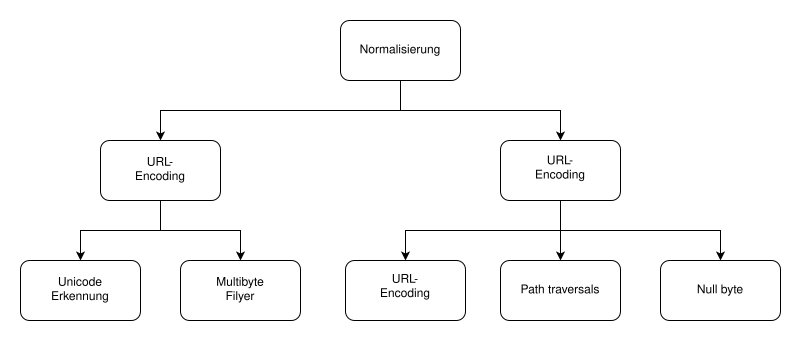
\includegraphics[width=0.9\textwidth]{./images/Normalisierung.png}
    \caption{Normalisierungsoperationen}
    \label{fig:norming}
\end{figure}

Normalisiert werden muss zum Einen die Zeichendarstellung.
Die Nachricht muss in ein einheilichs Encoding überführt werden, außerdem müssen \textit{URL-Encodings} aufgelöst werden.
Hier werden Sonderzeichen mit drei bytes dargestellt:
Das erste Zeichen ist immer ein \verb|%| gefolgt von einer Zahl in hexadezimaler Darstellung der das Zeichen repräsentiert.
Das \verb|@|-Zeichen wird von \verb|%40| repräsentiert, soll das Zeichen \verb|%| selber dargestellt werden muss dies mit \verb|%25| codiert werden.
Weitere Normalisierungsoperationen sind das Entfernen von Null Bytes.
Ein Null Byte ist ein Zeichen das nicht dargestellt wird.
Alle oben genannten Techniken können genutzt werden um nicht von regulären Ausdrücken erkannt werden zu können.

Eine weitere Gruppe von Normalisierungsoperationen sind Pfad-Normalisierungen.
Sollen Pfade nicht Normalisiert werden kann ein Angreifer Zugriff auf Verzeichnisse erlangen, die nicht zugänglich sein sollten.

Ist der Request Parsing Schritt abgeschlossen, liegt einen Nachricht in einer Form vor, die eine Einheitliche Analyse ermöglicht.

\paragraph{Muster-Abgleich gegen Regeln}
% - Abgleichen gegen Feature Datenbank
% - Jeder Parameter gegen jede regex
%     - Rechenaufwand
%         - optimierte regex-Engines
%         - Tree pruning
%             - Gefahr durch ungewollte pass on Szenarien
% - Whitelisting
%     - Features deaktivieren die web app-Funktion einschränken
% - Blacklisting
%     - Default Regelwerk
% - Auch Signatur-basierte WAFs
%     - komplexere Erkennung

Die normalisierte Nachricht kann von der \ac{waf} nun auf schädliche Inhalte untersucht werden.
In der Regel erfolgt das durch den Abgleich gegen eine Regel.
Eine Regel besteht aus einem regulären Ausdruck und einem Set an Instruktionen wie mit der Nachricht, im Fall das eine Übereinstimmung besteht, verfahren werden soll. 



\paragraph{Logging}
% - Jeder Schritt wird protokolliert
%     - Compliance
%         - Erfiltrierte Daten
%         - betroffene Nutzer
%     - Nachvollziehbarkeit von Fehlern
% - Log analyse
%     - Hauptarbeit eines WAF-Consultants

\paragraph{Weiteres Vorgehen}
% - Request Ablehnen
%     - Werden schädliche Daten erkannt
% - Request modifizieren
%     - Ablehnen bei schädlichen Inhalten nicht notwendig
%     - request kann umgeschrieben werden
%         - Abschnitte entfernen
%         - Abschnitte Escapeen
% - unmodofiziertes weiterleiten
% 
% - aus normalisierter form HTTP-Request erstellen
% - an server übergeben

\subsubsection{Erweiterte Funktionen}
\paragraph{Lernen von Regeln aus vorhergegangenem Datenverkehr}
\paragraph{KI-Features}
\subsubsection{Deployment einer WAF}
\paragraph{Postitionierung einer WAF}
\paragraph{Betrieb einer WAF}
\subsubsection{Schwächen und Nachteile einer WAF}

    \pagebreak

    \section{Design und Umsetzung der Lernumgebung}
    Dieses Kapitel beinhaltet die Beschreibung der Laborumgebung deren Erstellung eines der Hauptziele dieser Thesis ist.
Es werden zuerst Abwägungen zu den Inhalten, die übermittelt werden sollen, angestellt.
Des Weiteren werden Produkte evaluiert die für die Realisierung der Laborumgebung genutzt werden können und deren Nutzung in der Laborumgebung beschrieben.
Es wird sowohl eine \ac{waf} als auch eine Anwendung benötigt, die zu schützende Schwachstellen aufweist.
Final werden die erstellten lerneinheiten beschrieben und Abwägungen angestellt wie die Lerneinheiten die erarbeiteten Leerinhalte übermitteln können.

\subsection{Zielsetzungen und grundlegende Überlegungen}
\label{sec:learnings-metha}

%Wird eine \ac{waf} als Schutz einer Webanwendung eingesetzt unterscheidenden sich die Aufgaben die für den Betrieb ausgeführt werden müssen deutlich von den Inhalten, die 
% ToDo Waf wird in Vorlesung vorgestellt
% ToDO Zeitvorgabe
Der Fokus der Lerneinheiten soll auf der Funktion einer \ac{waf} liegen.
Die Lerneinheiten sind nicht geeignet um das Aufgabenfeld von \ac{waf}-Consultants zu vermitteln.
Der Fokus liegt auf dem Erkennen, Verstehen und abwehren von Cyber-Angriffen.
Im Betrieb einer \ac{waf} wird das hierfür notwendige Regelwerk mit den Produkten vorkonfiguriert ausgeliefert.
Die Aufgaben in diesem Fall sind die Reaktion und Adaption der \ac{waf} auf entstehende Fehler um die Nutzung der zu schütztenden Webseite ohne Funktions-Einschränkungen zu ermöglichen.

In der Laborumgebung sollen diese vorkonfigurierten Regeln von den Lernenden erarbeitet werden.
Die Entstehende Konfiguration ist höchst spezialisiert und kann in einem realen Szenario nicht ansatzweise Sicherheitsvorteile erbringen.
Die bei einer Produktiven-\ac{waf} mitgelieferten Regelwerke werden von Mathematikern oder Theoretischen Informatikern erstellt und sind deutlich Allgemeingültiger als diejenigen die in dieser Laborumgebung erarbeitet werden.\\

Die Lerneinheiten sind angelegt begleitend zu theoretischem Unterricht durchgeführt zu werden.
Parallel zu der Durchführung sollen die Lernenden das Wissen erhalten welches in den Grundlagen-Kapiteln (Kapitel \ref{sec:theoretical-foundations}) beschrieben ist.
Die Laborumgebung ist nicht dafür ausgelegt dies theoretischen Grundlagen zu vermitteln und stützt sich zu Teilen auf dieses Wissen.
Die Lerneinheit soll in einer Vorlesung mit 4 SWS innerhalb dreier Wochen durchführbar sein.
Das Heißt es werden pro Lerneinheit 3 bis 5 Stunden Zeitaufwand angesetzt.

Die Laborumgebung besteht aus drei, aufeinander aufbauenden Lerneinheiten.
In einem erste Schritt soll, nachdem sich mit dem Aufbau der Laborumgebung vertraut gemacht wird, die generelle Position einer \ac{waf} im Netzwerkverkehr beschrieben werden.
Es sollen unkompliziert zugängliche Inhalte des \ac{http}-Protokolls analysiert werden um den generellen Aufbau einer einer Regel und die schritte der Verarbeitung in einer \ac{waf} zu Verstehen.\\

Die Zweite Lerneinheit beschäftigt sich mit grundlegenden Angriffen die von einer \ac{waf} abgefangen werden können.
Hierfür werden einige grundlegende Schwachstellen herangezogen die sowohl in der Realität auftreten als auch ohne Vorkenntnisse mit Sicherheitslücken in Webanwendung verständlich sind.
Die benötigten Vorkenntnisse sollen nur im Bereich der Software-Entwicklung und der Erstellung von Webseiten sowie einem Grundverständnis des \ac{http}-Protokolls liegen.
Anhand dieser Kenntnisse und der Beschreibung von Schwachstellen in der zu schütztenden Webanwendung soll ich ein Verständnis der Angriffsvektoren erarbeitet werden und ein Regelwerk erstellt werden, das diese abdeckt und die Ausnutzung vereitelt.

Um neben dem Regelwerk auch einen Einblick in den betrieb einer \ac{waf} zu vermittel fokussiert sich die dritte Lerneinheit darauf mit einer \ac{waf} im alltäglichen Betrieb zu arbeiten.
Hier sollen die Lernenden mit einer Fehlerhaften \ac{waf}-Regel Konfrontiert werden, die das rechtmäßige Funktionieren der Webanwendung  hinter der \ac{waf} beschränkt.
Sie sollen diese Regel analysieren, mit den Folgen für die Netzwerkkommunikation beschäftigen und die Regeln adaptieren, sodas die Funktion der Webseite wiederhergestellt werden kann.
Des Weiteren soll die dritte Lerneinheit sich mit Techniken der Filter-evasion beschäftigen.
Hier sollen sich die Lernenden mit Techniken auseinandersetzen, die genutzt werden können um zu verhinder, dass ein Regulärer Ausdruck einen schädlichen Inhalt als solchen erkennt.
Solche Techniken werden in realen Angriffsszenarien an einem Filter vorbei Angriffe zu ermöglicht.
Eine \ac{waf} bietet auch für derartige Angriffe Verteidigungen.
    \subsection{Technische Umsetzung}
    \subsubsection{Evaluation verfügbarer Produkte}
\label{sec:produkt-eval}
\paragraph{Auswahl der \ac{waf}-Anwendung}

\paragraph{Verwundbare Anwendungen}

\subsubsection{Labor-Umgebung}

% 1. Anforderungen an die Lernumgebung
% 2. Überlegungen zur gestaltung einheiltichen Deployments
% 2.1. Docker
%       - einheitlich
%       - Netzwerke
%       - Probleme mit croscompatibility (Windows)
% 2.2. VM (vortiele und Probleme)
% 3. beschreibung der Container
% 3.1. Juicesop
% 3.2. WAF
% 3.3. Python contaienr mit test script

Die in Kapitel \ref{sec:inhalte} beschriebenen Inhalte sollen in einem Praxisnahen Umfeld vermittelt werden.
Dazu kommt nach den Abwägungen aus Kapitel \ref{sec:produkt-eval}, die Waf-Applikation ModSecurity zum Einsatz.
Die zu diesem Zweck vorgesehene Laborumgebung muss einige Kriterien erfüllen:
\begin{description}
    \item[Einheitliches Deployment:] Der Ausgangspunkt der Lerneinheiten muss reproduzierbar und wiederholbar sein. 
    Bei wiederholten Durchführungen der Übungen soll es einfach sein den Lernenden ohne zusätzlichem manuellen Konfigurationsaufwand eine Laborumgebung zu übergeben. 
    Diese Laborumgebung muss Platform-unabhängig aufgebaut sein und auf Windows, MacOS unf Linux genutzt werden können.
    \item[Modifizierbarketit der Anwendungen:] Um in den Lerneinheiten grundlegende Techniken zu übermitteln, ist es notwendig Basis-Funktion der ModSecurity \ac{waf} entfernen zu können. 
    Dies muss automatisierten und einheitlichen Weg erfolgen können.
    \item[Bekannte Basis-Technologien:] Der Fokus der Lerneinheiten liegt auf dem Erlernen der Technik und Funktion einer \ac{waf}. 
    Um einen Einstieg möglichst direkt zu gestalten sollen hierfür Technologien zuj Einsatz kommen, die den Lernenden schon bekannt sind und keinen zusätzlichen Lernaufwand erzeugen.
    \item[Komplexe Netzwerkumgebungen:] Da die verschiedenen Anwendungen in der Laborumgebung über Netzwerkkommunikation miteinander kommunizieren, muss es möglich sein automatisiert virtuelle Netzwerke zu erzeugen.
\end{description}

Um den oben genannten Anforderungen möglichst genau zu entsprechen, wurde die in Abbildung \ref{fig:lab} schematisch dargestellte Umgebung erstellt.

\begin{figure}[!hbt]
    \centering
    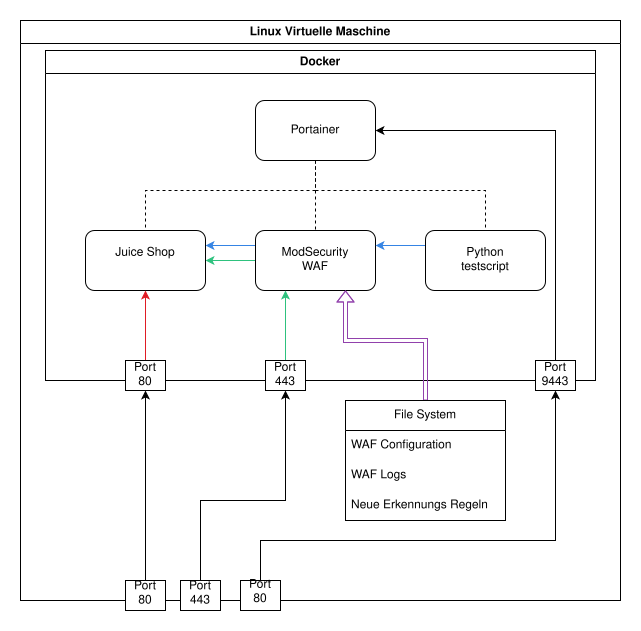
\includegraphics[width=0.9\textwidth]{./images/lab-setup.png}
    \caption{Aufbau der Laborumgebung}
    \label{fig:lab}
\end{figure}

Als Basis wird die Containervirtualisierungsumgebung Docker verwendet.
Diese ermöglicht es isolierte Ausführungsumgebungen für die Anwendungen zu erzeugen.
Der Aufbau dieser Umgebungen lässt sich mittels einer Konfigurationsdatei genau beschreiben und wiederholbar ausrollen.
Innerhalb der Umgebungen lässt sich festlegen wie die einzelnen Anwendungen (Container) untereinander kommunizieren und virtuelle Netzwerke anlegen um die Kommunikation zu isolieren.
Außerdem können Dateien oder Ordner aus dem Host-Dateisystem in den Container übergeben werden.
Dies ermöglicht es Konfigurationsdateien zu Verfügung zu stellen und somit, die sonst Status-losen Container, anzupassen.
Im Gegensatz zu virtuellen Maschinen greift die Containervirtualisierungsumgebung direkt auf die Mittel des Host-Betriebssystem zu und benötigt dadurch deutlich weniger Rechenaufwand.\\
\ \\
Wie in Abbildung \ref{fig:lab} dargestellt werden in der Laborumgebung vier Container betrieben:
\begin{description}
    \item[ModSecurity \ac{waf}:] Der Hersteller der in der Laborumgebung verwendeten \ac{waf} - ModSecurity - stellt sein Produkt auch in Form eines Docker-Containers zur Verfügung. 
    Diese wird jedoch in modifizierter Form genutzt.
    Da die \ac{waf} mit einer großen Anzahl vorkonfigurierten Regeln ausgeliefert wird, die für die meisten Aufgaben schon eine Lösung enthalten würden, müssen diese entfernt werden.
    An dessen Stelle wird ein Verzeichnis aus dem Host-Dateisystem durchgereicht in dem die Lernenden eigene Konfigurationen Platzieren können.
    Daneben werden, um das Debugging zu ermöglichen, die Log-Dateien aus der \ac{waf} im Host betriebssystem zur Verfügung gestellt.ds
    
    \item[Juice Shop:] Dieser wird in Version 16.0.0 verwendet, da der Hersteller (OWASP) die Anwendung regelmäßig verändert.
    Durch die Verwendung der neuesten Version könnten Challenges verloren gehen, die für die Durchführung der Aufgaben notwendig wäre.
    Auch diese Anwendung wird in modifizierter Form Ausgeliefert.
    Es werden Daten hinterlegt und Nutzeracounts angelegt.
    Diese ermöglichen es Mittels eines automatischen Kontroll-Scriptes die Konfiguration der \ac{waf} zu überprüfen.
    Die genauen Änderungen werden in den Sub-Kapiteln von Kapitel \ref{sec:learnings} im Detail beschrieben.

    \item[Python Test-Script:] Dieser Container enthält ein Python Skript, das es den Lernenden mittels des Unittest-Frameworks \textit{Pytest} ermöglicht, die erarbeiteten Lösungen zu überprüfen.
    Das Skript schickt HTTP-Requests durch die \ac{waf} und evaluiert die Antworten um den Lernenden Rückmeldung über den Erfolg ihrer Kofiguyration zu geben.
    Die jeweilige Funktion wird in den Sub-Kapiteln von Kapitel \ref{sec:learnings} im Detail beschrieben.

    \item[Portainer:] Die Anwendung \textit{Portainer} ermöglicht es eine Docker Umgebung mittels einer Grafischen Oberfläche zu verwalten.
    In der Laborumgebung kann sie genutzt werden um die Laborumgebung zu bedienen ohne sich tiefer mit der Funtion von Docker auseinander setzen zu müssen.
    Zwar können die Lernenden dies auch über das Docker Komandozeilen-Interface tun, jedoch beurteile ich dies als eine vermeidbare Hürde, die den Einstieg erschweren könnte.
    Die grafische Oberfläche soll unter anderem genutzt werden um des \ac{waf} kontainer nach einer Konfigurationsänderung neu zu starten und mit dem Test Skript zu interagieren. 
\end{description}
\ \\
Aus den oben genannten Containern ergeben sich einige Netz die im Hintergrund existieren müssen.
So ist es notwendig das von dem Python Test-Container zur \ac{waf} und von dieser eine Verbindung zum Jucice Shop aufgebaut werden muss.
Hierfür werden separate Docker-Netzwerke erstellt die an den Containern angeschlossen sind.
Um den Nutzern eine Interaktion mit den Containern zu ermöglichen werden einige Ports aus der Docker-Umgebung freigegeben:

\begin{itemize}
    \item Die Web-Oberfläche des Juice Shops (Port 80 [HTTP])
    \item Die, durch die \ac{waf} gesicherte, Web-Oberfläche des Juice Shops (Port 443 [HTTPS])
    \item Das Management Interface der Portainer-Anwendung (Port 8443 ][HTTPS])
\end{itemize}

Durch die oben beschriebene Docker Umgebung sind Anforderungen an die Laborumgebung wie dem \textit{einheitlichen Deployment} und der \textit{Modifizierbarketit der Anwendungen} bereits erfüllt.
Es ergeben sich jedoch auch einige Herausforderungen:
Docker ist zwar als Cross-Platform Anwendung konzipiert.
Es stehen Versionen für die drei Gängigen Betriebssysteme Windows, MacOS und Linux zur Verfügung.
Jedoch bauen die verwendeten Container Hauptsächlich auf Linux auf.
In der Theorie sollte dies zu keinen Problemen führen, da Docker in der Lage ist nicht Platform-Native Container auf sich unterscheidenden Betriebssystemen auszufühen, jedoch kann ein solcher Aufbau durchaus zu unvorhergesehenen Problemen führen.
Ein weiteres Problem ist, dass durch das Durchreichten von Dateien zwischen Container und dem Host-Dateisystem zusätzlicher Konfigurationsaufwand für die Nutzer entsehen könnte.

Um diesen Problemen Vorzubeugen wird die Laborumgebung als Linux Virtuelle Maschine ausgeliefert.
In dieser ist eine Docker Umgebung vorinstalliert und die Containerumgebung bereits präsent und wird automatisch gestartet.
Dies ermöglicht die Auslieferung mittels einer VM-Datei, in der die Konfigurationen schon an einer einheitlichen Stelle enthalten sind.
Lernende müssen zur Nutzung also nur eine Virtuelle Maschinen auf ihren Rechnern importieren und mittels eines Virtuellen Netzwerk Interface auf die Web-Oberflächen zugreifen.
Die Konfiguration der \ac{waf} findet in Textdateien statt, die sich in der Virtuellen Maschine befinden.
Der Zugriff auf diese ist mit dem Text-Editor Visual Studio Code der Firma Microsoft vorgesehen, da dieser eine SSH Erweiterung hat die es mit geringen Konfigurationsaufwand ermöglicht Dateien auf entfernten Servern oder in Virtuellen Maschinen zu bearbeiten.

Die Nutzung der Laborumgebung halte ich durch diese Maßnahmen für einfach genug um einen schnellen einstieg zu Ermöglichen.
Die Konfigurationen, die vorgenommen werden müssen, werden in der Ersten Lerneinhiet (Kapitel \ref{sec:lerneinheit1}) Beschrieben.
Es steht den Lernenden frei weitere oder andere als die beschriebenen Technologien zu verweden um mit der Laborumgebung zu interagieren.
Diese können im Rahmen dieser Thesis und den Aufgabenstellungen jehdoch nicht berücksichtigt werden.

\pagebreak
    \subsection{Lerneinheiten}
    \label{sec:learning-unit-meta}
    Die in diesem Kapitel beschriebenen Lerneinheiten machen in der praktischen Arbeit einen zentralen zentralen Bestandteil dieser Thesis aus.Sie ähneln sich in Aufbau und Durchführung, beschäftigen sich jedoch mit unterschiedlichen Aspekten einer \ac{waf}:
Eine Aufgabe in einer Lerneinheit beginnt immer mit einigen Worten zu dem Thema mit dem sich die Lernenden beschäftigen sollen, gefolgt von einer Referenz auf eine Challenge aus dem Juice Shop die mit der \ac{waf} abgesichert werden soll.

In diesem Kapitel wird beschrieben welche Überlegungen in die Konzeption der Lerneinheit geflossen sind.
Mit welchem Oberthema sich die jeweiligen Lerneinheiten beschäftigen, nach welchen Kriterien die Challenges des Juice Shops ausgewählt wurden und wie die Challenges gelöst werden können.

\subsubsection{Teil 1: Erster Kontakt zu einer WAF}
\label{sec:learning-unit-1-meta}

In der ersten Lerneinheit sollen sich die Lernenden mit der Laborumgebung vertraut machen.
Erst sollen die Lernenden die Laborumgebung auf ihren Geräten einrichten und sich versichern, dass sie Zugriff auf alle Services der Umgebung haben.
Dann gilt es ein Verständnis aufzubauen wie der Fluss einer \ac{http}-Anfrage durch die Netzwerke der Umgebung erfolgt.
Den Lernenden sollte vor Beginn der Lerneinheit bekannt sein wie eine \ac{waf} in der Theorie vor eine Webanwendung platziert werden kann.\\

Die eigentlichen Aufgabenstellungen zu der hier beschrieben Lerneinheit sind in Anhang \ref{sec:learning-unit-1} zu finden.\\

\paragraph{Einrichtung der Laborumgebung}\ \\

In der ersten Aufgabe (Anhang \ref{sec:learning-unit-1-preparations}) der Lerneinheit sollen die Lernenden die Laborumgebung installieren.
Hierfür muss die die \ac{vm} der Laborumgebung bereit gestellt werden.
Die weiteren Anwendungen, die im Zuge der Durchführung benötigt werden, werden in der Aufgabenstellung genannt und die Konfiguration erläutert.
Die Aufgabe besteht aus einer detailliert bebilderten Anleitung zum Aufsetzen der Laborumgebung.
Die Bestandteile sind:

\begin{enumerate}
    \item Installation der \ac{vm}
    \item Konfiguration eines virtuellen \textit{Host-Only} Netzwerkadapters um vom Host Betriebssystem auf die \ac{waf}-Laborumgebung zugreifen zu können.
    \item Abrufen der Verfügbaren Webanwendungen
    \item Verbinden mit der SSH-Schnittstelle um die \ac{waf} Konfiguration bearbeiten zu können.
\end{enumerate}

Die Anleitung ist mit dem Fokus auf einige notwendige und empfohlene Technologien verfasst.
Es wird nur die gängigste Methode beschrieben die Laborumgebung aufzusetzen: Windows und VirtualBox.
Es wird jedoch auch auf einer konzeptionellen Ebene beschrieben, was zu tun ist.
Lernende, die andere als die beschrieben Technologien nutzen möchten, können dies tun, dies ist in der Konzeption der Laborumgebung berücksichtigt, wird in der Anleitung aber nicht genauer beschrieben.
Lernende die sich dafür entscheiden müssen auftretende Probleme mit den von ihnen gewählten Technologien eigenständig und ohne Hilfe der Anleitung lösen.

Nach Abschluss der Aufgabe müssen die Lernenden in der Lage sein, die Laborumgebung zu nutzen um weitere Aufgaben zu lösen.
Die Lernenden müssen sich nur in geringem Maße neues Wissen erarbeiten, da die Anleitung sehr eng geführt ist.

\paragraph{Erste Arbeit mit der WAF}\ \\

In dieser Aufgabe in der sich die Lernenden das erste Mal mit \ac{waf}-Regeln beschäftigen.
Für den Einstieg soll sich zuerst mit der Syntax der \textit{ModSecurity} Regeln anhand einfacher Beispiele beschäftigt werden.
Hierfür werden zwei Challenges des \textit{Juice Shops} herangezogen deren Lösungen ohne größere Probleme nachvollziehbar sind.
In der Ersten dieser Aufgaben soll ein Pfad unzugänglich gemacht werden, auf dem sensitive Informationen preisgegeben werden.
Die hierfür notwendige Regeln ist verhältnismäßig unkompliziert und kann beispielsweise wie Folgt aussehen:

\begin{verbatim}
SecRule REQUEST_URI "@streq /ftp/acquisitions.md" \
    "id:1, \
    msg:'Stop access to critical /ftp/aquisitions.md', \
    deny, \
    status:403"
\end{verbatim}

Der zweite Teil der Aufgabe erfordert es, den Inhalt eines \ac{http}-Bodies zu parsen und zu analysieren.
Die zugehörige Challenge im \textit{Juice Shop} weist eine Schwachstelle auf, in der Parameter im Backend nicht auf Gültigkeit geprüft werden.
Dadurch können ungültig Daten an den Webserver übergeben werden, die dort gespeichert und von dort an Nutzer übergeben werden.
Der Parameter \textit{rating}, der in einem JSON-Objekt im \ac{http}-Request Body transportiert wird soll nur die Werte 1 bis 5 annehmen können.

Der schädliche Parameter kann auf unterschiedlichen Wegen erkannt werden.
Zwei Beispiele wären:\\

\begin{itemize}
    \item Mithilfe eines regulären Ausdrucks ($[\land 1-5]$):
    \begin{verbatim}
    SecRule REQUEST_HEADERS:Content-Type "application/json" \
        "phase:2, id:3, t:none, t:lowercase, \
        log, ctl:requestBodyProcessor=JSON" \
        chain, \
        msg:'JSON parameter rating found in request body'"
    
        SecRule REQUEST_BODY:rating "@rx [^1-5]" \
            "id:4, phase:2, \
            deny, log, status:403"
    \end{verbatim}

    \item Mithilfe von Vergleichsoperationen (\textit{@gt 5} und \textit{@lt 1}):
    \begin{verbatim}
    SecRule REQUEST_HEADERS:Content-Type "application/json" \
        "phase:2, id:3, t:none, t:lowercase, \
        log, ctl:requestBodyProcessor=JSON" \
        chain, \
        msg:'JSON parameter rating found in request body'"
        
        SecRule ARGS:rating "@gt 5" \
            "id:4, phase:2, \
            deny, log, status:403"
    
        SecRule ARGS:rating "@lt 1" \
            "id:5, phase:2, \
            deny, log, status:403"
    \end{verbatim}
\end{itemize}

Diese Challenges sollen den Lernenden grundlegende Konzepte zum Aufbau einer \textit{ModSecurity} Regel beibringen:
\begin{itemize}
    \item Den grundlegenden Aufbau nach der Struktur
    \begin{verbatim}
        SecRule VARIABLE [OPERATOR] [TRANSFORMATIONS,ACTIONS]
    \end{verbatim}
    in der erst das Ziel der Operation (VARIABLE), dann die Matching-Operation (OPERATOR) und dann das Verfahren nach dem \textit{Match} (TRANSFORMATIONS,ACTIONS) beschrieben werden.
    \item Das Prinzip des \textit{Multi Stage Processing}: Nicht die ganze \ac{http}-Nachricht steht zur gleichen Zeit zur Verfügung. Der Zugriff auf ein JSON-Body Element kann, wie in dem Beispiel oben, also erst nach vorherigem Parsing betrachtet werden.
\end{itemize}

Die beiden oben beschrieben Aufgaben sind gedacht, um die \ac{waf} kennen zu lernen.
Sie bilden jedoch kein Verhalten ab das in einer \ac{waf}-Regel einer produktiven \ac{waf} verwendet werden würde:
Die Regeln sind viel zu detailliert und auf einen spezifischen Fall ausgerichtet.

\subsubsection{Teil 2: Grundlegende Angriffe}
\label{sec:learning-unit-2-meta}

Nachdem sich in der ersten Lerneinheit mit der Laborumgebung, der \ac{waf} und ihrer Funktion vertraut gemacht wurde, kann der Fokus in dieser zweiten Lerneinheit auf Angriffsszenarien gelegt werden.
Die Lernenden beschäftigen sich exemplarisch mit zwei Angriffsszenarien, die in der aktuellen IT-Sicherheit und Verteidigung von Webanwendungen relevant sind.\\

Die Aufgabenstellungen zu der hier beschreiben Lerneinheit sind in Anhang \ref{sec:learning-unit-2} zu finden.

\paragraph{SQL Injections}\ \\
Die SQL-Injection ist eine Angriffstechnik bei der Nutzereingaben direkt und ungefiltert an eine SQL-Datenbank im Backend weitergegeben werden.
Dies kann zu unvorhergesehenen Nebeneffekten wie Befehlsausführung auf dem Server und Daten-Exhilaration führen.
Nach \textit{OWASP-Top-Ten} gehören SQL Injections zu den zehn schwerwiegendsten Schwachstellen, die in Webanwendungen zu finden sind.

Die Funktion und Verteidigung gegen SQL Injection Angriffe sollen Lernenden in dieser Aufgabe erarbeiten.
Zuerst soll sich mit einer spezifischen Sicherheitslücke beschäftigt werden und diese mit einer eigenständigen \ac{waf}-Regel mitigiert werden.
In einem zweiten Schritt wird einen SQL-Injection generell betrachtet.
Hierfür sollen die Lernenden die Gemeinsamkeiten von zwei \textit{Juice Shop} Challenges herausarbeiten und beide Schwachstellen mit einer Regel mitigieren.

Die erste Teilaufgabe beschäftigt sich mit einem SQL Login-Bypass.
Zum Abgleich, ob ein Nutzer existiert und das Passwort gültig ist, wird im Backend die SQL-Datenbank genutzt.
Ein Angreifer kann in dieser \textit{Juice Shop} Challenge an den Nutzernamen einen Vergleich in SQL Syntax anhängen und somit einen gültigen Login erzwingen ohne das Passwort eines Nutzers zu kennen.

Um diesen Angriff erkennen zu können, sollen sich die Lernenden auf escape syntax fokussieren, mit deren Hilfe ein SQL-Befehl beendet werden kann, um danach eigene Befehle auszuführen.

Zwei Beispiele könnten wie Folgt aussehen:

\begin{verbatim}
SecRule ARGS:email "@rx ^['].*--" \ 
    "id:6, phase:2, \
    deny,log,status:401"

SecRule ARGS:email "@rx ==\w*--" \
    "id:7, phase:2, \
    deny,log,status:401"
\end{verbatim}

In beiden Fällen wird nach dem Beginn eines SQL Kommentars gesucht.
Die beiden dargestellten Möglichkeiten suchen vor dem Kommentar jedoch nach unterschiedlichen Angriffsmustern.
Im ersten Beispiel werden Hochkommata gemacht, die in einer Mailadresse nicht vertreten sein sollten.
Im zweiten Fall wird nach einem Vergleich ($==$) gesucht, der zwar theoretisch in einem nicht bösartigen Szenario vorkommen könnte, jedoch eher unwahrscheinlich ist und keine Einschränkung für Nutzer darstellen würde.
Der \ac{http}-Error-Code der in diesen Beispielen zurückgegeben wird unterscheidet sich zu denen, die in den Regeln aus Aufgabe 1 (siehe Kapitel \ref{sec:learning-unit-1-meta}) vorkommen.
Dies liegt an der unterschiedlichen Situation:
In diesem Beispiel handelt es sich um Fehlende Autorisierung eine Anfrage zu machen:
Der status code 401 (Unauthorized) wird gewählt.
Im vorherigen Beispiel ist der Zugang zu der Resource generell verboten: der status code 403 (Forbidden) wird gewählt.

Im zweiten Teil der Aufgabe soll sich nun auf das generelle filtern von SQL-Syntax fokussiert werden.
Die beiden Challenges die die Lernenden analysieren sollen weisen SQL-Injection Schwachstellen im HTTP-Body auf.
Damit die Lernenden keine Regeln schreiben können, die sich nur auf einen spezifischen Fall beschränkt sollen die Lernenden eine Regel für beide Challenges schreiben.

Ein Lösungsvorschlag für das generelle Erkennen einer SQL-INjection Attacke kann sein die sql keywords zu erkennen wie in dem folgenden regulären Ausdruck nachvollziehbar ist.

\begin{verbatim}
\s*(select|union|update|delete|insert|drop|--|or|and|alter|exec
|create|script|table|from|where|join|having|cast)\s*
\end{verbatim}

Beim schreiben der Regel müssen die Lernenden darauf achten, dass die Regel keine unvorhergesehenen Nebeneffekte hat.
Wird beispielsweise nur nach dem substring \verb|and| gefiltert, könnte ein Nutzer mit dem Namen \textit{Andy} Probleme bekommen die Webanwendung zu nutzen.\\


Ist die Aufgabe abgeschlossen sollen die Lernenden ein Verständnis dafür haben wie eine SQL-Injection Funktioniert.
Außerdem sollen sie durch das lösen von Problemen und betrachten der Logs herausgefunden haben, dass ein regulärer Ausdruck dessen Folgen nicht bedacht wurde Probleme bei der regulären Nutzung der Webanwendung hervorrufen kann.

\paragraph{Cross Site Scripting (XSS)}\ \\

Neben der \textit{SQL-Injection} nutzen Angreifer häufig sogenannte \ac{xss} Schwachstellen in Webanwendungen aus.
Bei einem \ac{xss} ist es einem Angreifer möglich HTML und Java Scrip Code an die Webanwendungen zu übergeben sodass dieser von der Anwendung nicht als Text interpretiert wird sonder als Code Ausgeführt bzw. dargestellt wird.

In diesem Teil der Lerneinheit sollen sich die Lernenden mit der Funktion einer \ac{xss} Schwachstelle vertraut machen und daraus ableiten, wie ein solcher Angriff erkannt und verhindert werden kann.
Des weiteren besitzen Browser Funktionen die das Ausnutzen eines \ac{xss} erschweren.
Diese werden können in einem HTTP request durch das Setzen eines bestimmten Headers oder dem erstellen einer \textit{Content Security Policy} die festlegt von welchen Quellen Daten nachgeladen werden dürfen.
Dies kann auch durch die \ac{waf} erfolgen.
An diesem Beispiel ist es auch möglich das Umschreiben eines \ac{http}-Request durch die \ac{waf} zu übermitteln.

Im ersten Teil der Aufgabe sollen die Lernenden eine \ac{waf}-Regel schreiben die in eingehendem Traffic ein HTML-Tag und javascript erkennt und Blockiert.
Es existieren mehrere Möglichkeiten einen solchen Angriff zu erkennen und abzuwehren.
Anhand der öffnenden und schließenden HTML-Tags oder dem \textit{javascript} Tag.
Im folgenden beispiel ist eine Möglichkeit dies anhand der HTML \textit{script Tags} zu tun dargestellt:

\begin{verbatim}
    SecRule REQUEST_HEADERS:Content-Type "application/json \
        [...]
        SecRule ARGS: "@rx <script[^>]*>.*</script>|<[^>]+>" \
        [...]
\end{verbatim}

Für eine allgemeine Lösungen nicht hinreichende, jedoch in dem spezifischen Fall der Übung gültige Lösung wäre das erkennen des javascript codes.
Das Hierfür zum Testen genutzte \textit{javascript:alert} ist austauschbar und würde keinen zuverlässigen Schutz sorgen.

Der Zweite Teil der Aufgabe beschäftigt sich mit dem mit dem setzen des \textit{X-XSS-Protection} Headers.
Hierfür muss in einer Regel ausgehender Netzwerkverkehr erkannt werden.
Anstatt diesen zu blockieren kann der Header gesetzt werde, wie im Folgenden Beispiel zu sehen ist:

\begin{verbatim}
SecRule RESPONSE_HEADERS:@streq 200 \
   "id:10, phase:3, nolog, pass,\
   hdrOut: Header set X-XSS-Protection '1; mode=block'"
\end{verbatim}

Die Lernenden sollen nach Abschluss dieser Lerneinheit ein Verständnis für die Funktion eines \ac{xss} haben.
Außerdem soll ein Bewusstsein für die Funktion der \ac{xss}-Protection Header bestehen, die einen wichtigen ersten Verteidigungsschritt gegen diese Angriffe darstellen.
Neben dem Verständnis für den Angriff wird auch die Fähigkeit einer \ac{waf} den Netzwerkverkehr nicht nur zu bloc sonder auch umzuschreiben vermittelt.

\subsubsection{Teil3: Nutzung einer WAF in produktivem Umfeld}
\label{sec:learning-unit-3-meta}

Die dritte Lerneinheit soll einen Fokus auf der Arbeit mit einer \ac{waf} in produktivem Umfeld Legen.
Die Lernenden sollen mit den Logdateien arbeiten um den Fehler in einer \ac{waf}-Regel zu finden.
Außerdem ist vorgesehen, dass sich die Lernende mit Techniken der \textit{Filter evasion} beschäftigen, die ein Angreifer Nutzen könnte um nicht von den regulären Ausdrücken einer \ac{waf} erkannt zu werden.\\

Im Rahmen der Thesis war es aus Zeitlichen gründen diese dritte Lerneinheit zu realisieren.

    \pagebreak

    \section{Evaluation}
    Um einschätzen zu können wie die Lerneinheiten in der Lehre eingesetzt werden könne wird eine Evaluation durchgeführt.
Wie viel Zeit wird für die Durchführung der Übungen benötigt?
Welche Vorkenntnisse sind notwendig um die Übungen erfolgreich durchführen zu können?
Welches wissen erwerben die Lernenden in der Laborumgebung?

Bevor die Laborumgebung begonnen wird, soll eine Selbsteinschätzung durchgeführt werden in der die Kenntnisse zu bestimmten Technologien abgefragt werden, die in der Laborumgebung relevant sind.
Die Teilnehmer sollen auf einer Skala von 1 bis 6 ihre Fähigkeiten in den folgenden Technologien bewerten:

\begin{itemize}
    \item Linux
    \item Virtuelle Maschinen
    \item Containervirtualisierungsumgebung Docker
    \item Softwareentwicklung
    \item Reguläre Ausdrücke
    \item HTTP auf Protokollebene
    \item SQL-Syntax
    \item Sicherheitslücken in Webanwendung
    \item Web Application Firewall
\end{itemize}

Nach der Selbsteinschätzung werden die Lerneinheiten durchgeführt.
Die Probanden sollen die Lerneinheiten eigenständig bearbeiten damit das Umfeld möglich nah an dem geplanten Einsatzgebiet der Laborumgebung ist.



\subsection{Evaluation mit Probanden}

Die Evaluation 

% Zeit
% Scheitern 
% da war noch was drittes



    \subsection{Überlegungen zur Bewertung der Lernenden}
    Als Teil der Thesis wird sich mit der Frage beschäftigt, wie eine Bewertung der Ergebnisse, die die Lernenden in der Laborumgebung erarbeiten, erfolgen kann.
Kann erkannt werden ob lernende Lösungen untereinander austauschen?
Es wird auch die Möglichkeit untersucht ob es möglich ist, die Laborumgebung so dynamisch zu generieren, dass die Laborumgebungen für jeden Lernenden einzigartig gestaltet ist.
Dies ließe sich beispielsweise durch dynamisch generierte Netzwerk-Topologien erreichen.
Einen weitere Möglichkeit wäre, jedem Lernenden unterschiedliche zu schützenden Challenges des \textit{Juice Shops} zuzuweisen.
Beide Ansätze stellen sich in der Durchführung der Thesis als nicht oder nicht innerhalb der Zeitvorgabe umsetzbar heraus.\\

%% ToDo bewertungh mitr abgabe
    \pagebreak


    \section{Fazit}
    Der Bereich der Cybersicherheit oft als eine Einheit wahrgenommen wird besteht er heutzutage aus einer weiten Auswahl an Technologien und Spezialgebieten, die alle einen wichtigen Beitrag zum sicheren Betrieb von IT-Systemen leisten.
Die Verschiedenen Felder benötigen alle qualifiziertes Fachpersonal um diese Sicherheit garantieren zu können.
%ToDo
Aus diesem Grund soll in dieser Thesis Lerneinheiten Entwickelt werden die in der Lehre eingesetzt werden kann um die Funktion einer \ac{waf} zu vermitteln.

\subsection{Zusammenfassung}
Das Ziel dieser Arbeit ist es Lerneinheiten zu erstellen mit deren Hilfe es Lernenden möglich ist einen Einblick in die Funktion einer \ac{waf} zu vermitteln.
Die Lernenden sollen, nachdem sie die Lerneinheiten bearbeitet haben, ein Verständnis dafür haben wie eine \ac{waf} im Netzwerkverkehr zwischen Server und Client platziert ist um ihre Sicherheitsfunktion zu erfüllen.
Es soll ein Tiefer Einblick in die Implementierung einer \ac{waf} vermitteln werden, besonders wie es mithilfe von Regeln möglich ist Netzwerkverkehr zu analysieren und schädliche Inhalte zu erkennen.
Dadurch sollen die Lernenden ein Verständnis dafür erlagen welche gängige Taktiken Angreifer nutzen um Schwachstellen in Webanwendungen auszunutzen.
Daraus soll sich das Wissen erarbeitet werden wie die Verteidigung gegen diese möglich ist.
Des weiteren sollen die Lernenden einen Einblick erhalten wie der Einsatz einer \ac{waf} in produktivem Umfeld erfolgen.
Die Lernenden sollen erfahren wie eine \ac{waf} in einem Netzwerk platziert wird um eine Webanwendung abzusichern und welche Tätigkeiten im betrieb einer \ac{waf} notwendig sind.

Im Ramen dieser Thesis wurde eine Laborumgebung Implementiert in der Lernende Aufgaben erfüllen können.
Anhand der Aufgaben wird den Lernenden aufeinander aufbauend die im vorherigen Abschnitt beschriebenen Inhalte vermittelt.
Um eine Abschätzung wie Lernende mit der Laborumgebung interagieren und wie erfolgreich die vorgesehenen Inhalte übermittel werden, wurde eine Evaluation der Laborumgebung mit Probanden durchgeführt.\\

Die Laborumgebung wird in Form einer Virtuellen Maschine ausgeliefert um die Durchführung möglichst Betriebssystem-Agnostisch zu ermöglichen.
In der Laborumgebung werden einige Services in Form von Docker-Containern zur Verfügung Gestellt.
Zum einen wird die verwundbare Webanwendung \textit{OWASP Juice Shop} betrieben.
Dies ist eine Open Source Webanwendung die mit Absicht Sicherheitslücken enthält und zu Ausbildung von Sicherheitsexperten oder Sensibilisierung für Schwachstellen genutzt werden kann.
Der zweite Service stellt mit der \ac{waf} \textit{ModSecurity} den Kern der Laborumgebung dar.
Es handelt sich um eine Open Source Anwendung, aus der das gesamte Regelwerk entfernt ist.\\

Die Lerneinheiten sind in drei Abschnitte unterteilt.
Der erste Abschnitt führt Lernende in die Laborumgebung und die Arbeit mit dem \textit{ModSecurity} Regelwerk ein.
Die Lernenden setzen angeleitet die Laborumgebung auf ihren Rechnern auf und interagieren mit den Services um ein Verständnis für die Umgebung bekommen.
In dieser Lerneinheit soll ein erstes Verständnis für das Schreiben und die Syntax der \ac{waf}-Regeln aufgebaut werden.
Nachdem sich die Lernenden mit der Laborumgebung vertraut gemacht haben, kann in der zweiten Lerneinheit begonnen werden angriffe zu Verstehen und abzuwehren.
Dies wird exemplarisch an den beiden Schwachstellen-Kategorien \textit{SQL-Injection} und \textit{Cross Site Scripting} durchgeführt.
Es wird erst exemplarisch auf einzelne Schwachstellen im \textit{Juice Shop} verwiesen, anhand derer in die Funktion der Angriffe eingeführt wird und Regeln zum expliziten mittigieren dieses einen Angriffs verfasst.
Danach sollen die Schwachstellen allgemein betrachtet werden und anhand von einer Auswahl an Schwachstellen ein Schutz mithilfe einer Einzelnen Regel erstellt werden.
Nach dem Verständnis für angriffe wird in der dritten Lerneinheit der Blick auf erweiterte Techniken und die Arbeit mit einer \ac{waf} gewendet.
Die Lernenden sollen sich in dieser Lerneinheit mit dem Härten von Filterregel beziehungsweise dem Umgehen von Filterregeln beschäftigen.
Des Weiteren soll mit den Log-Dateien gearbeitet werden um Fehler in der Konfiguration einer \ac{waf} aufzuspüren und diese zu Reparieren.
Im Ramen der Thesis war es aus zeitlichen Gründen nicht möglich diese Dritte Lerneinheit zu realisieren.\\

Die Laborumgebung wurde nach erstellen mit der Hilfe von Probanden Evaluiert um des Einsatz mit Lernenden Einschätzen zu können.
Ergebnisse sind zum einen, dass für die Durchführung ein Vorwissen in den Bereichen Reguläre Ausdrücke, der Funktion des \ac{http}-Protokolls und der Datenbanksprache SQL nötig sind.
Die Durchführung der Lerneinheiten kann von einem Lernenden in Ungefähr acht Arbeitsstunden erfolgen.
Von der Dauer her ist also ein Einsatz im Ramen einer Vorlesung möglich.

\subsection{Ausblick}

Diese Arbeit bietet einige Möglichkeiten weitere Überlegungen anzustellen und Erweiterungen vorzunehmen.

Zum Einen ist es für die tatsächliche Nutzung in der Lehre notwendig die Dritte und fehlende Lerneinheit zu Implementieren um die vorgesehene Lernerfahrung bieten zu können.
Es ließe sich beispielsweise den Lernenden ein Regelsatz für eine bestimmte Schwachstelle des \textit{Juice Shops} zur Verfügung stellen.
Diese Regelsatz müsste so gestaltet sein, dass die Funktion die eigentlich an dieser Stelle steht nicht verfügbar ist und nur durch das Umschreiben der Regeln ermöglicht werden kann.

Neben den fehlenden Inhalten existieren einige Punkte in denen noch weitere Arbeit betrieben werden kann um den Lernerfolg oder die Arbeit mit der Laborumgebung zu optimieren.
Als Teil der Laborumgebung ist es möglich einen Service zu Implementieren der den Lernenden mittels \ac{http}-Anfragen und Analyse der Antworten rückmeldung über die Qualität der erstellten Regeln geben kann.
Die Umsetzung eines solchen Services war als Teil der Laborumgebung geplant, in der vorgegebenen Zeit lies sich dies jedoch nicht zuverlässig Implementieren.
Die rückmeldung an die Lernenden war nicht von einer nutzbaren Qualität.

Weiter Überlegungen können außerdem zur Bewertung der Ergebnisse angestellt werden.
Kann die Laborumgebung prozedural so generiert werden, dass es möglich ist zu erkennen ob die Lernenden ihre Lösungen untereinander getauscht haben.
Dies wäre beispielsweise durch individuelle Aufgabenzuteilung möglich, sodass jeder Lernenden individuelle aufgaben hat.

%% automatische eval
    \pagebreak

    \pagebreak
\section{Bibliografie}
\label{sec:biblografie}

\printbibliography[heading=none]{}
    \pagebreak

    \appendix
    \section{Aufgabenstellung Teil I}
    \label{sec:learning-unit-1}
    Mit dieser Laborumgebung soll die Funktion einer Web Application Firewall (WAF) in drei Lerneinheiten vermittelt werden.
In dieser Lerneinheit sollen Sie sich mit der Lernumgebung vertraut machen und eine erste Konfiguration der WAF vornehmen.

\subsection{Vorbereitungen}
\label{sec:learning-unit-1-preparations}

Um die Laborumgebung zu nutzen werden die Folgenden Anwendungen benötigt:
\begin{itemize}
    \item \href{https://www.virtualbox.org/}{\underline{VirtualBox}}
    \item \href{https://code.visualstudio.com/download}{\underline{Visual Studio Code}}\\
    Die nicht quelloffene Version von Microsoft ist notwendig, da ein benötigtes Plugin in \textit{Open-Source} Distributionen wie \textit{vscodium} nicht verfügbar sind.
    \item Einen Web-Browser
\end{itemize}

\subsubsection{Virtuelle Maschine starten}
Importieren Sie nun die Virtuelle Maschine (VM),  die die Laborumgebung enthält in die VirtualBox Umgebung.
Die Datei (\textit{WAF-Laborumgebung.ova}) finden Sie im Moodle.

Bevor die VM gestartet werden kann, muss ein Host-Only Netzwerkadapter erstellt werden, um von ihrem Host-System auf die Services in der VM zugreifen zu können.
Die VM soll auf der IP-Adresse \textbf{192.168.56.2} aufrufbar sein.

Die folgende detaillierte Anleitung ist exemplarisch für Windows Systeme.
Wenn Sie ein anderes Betriebssystem oder eine andere Virtualisierungsumgebung nutzen, können Sie die Anleitung als Orientierung nutzen und müssen sich den Rest eigenständig erarbeiten.

\begin{enumerate}
    \item Den Netzwerk-Manager von VirtualBox aufrufen (\textit{File -> Tools -> Network Manager}).
    \begin{figure}[!hbt]
        \centering
        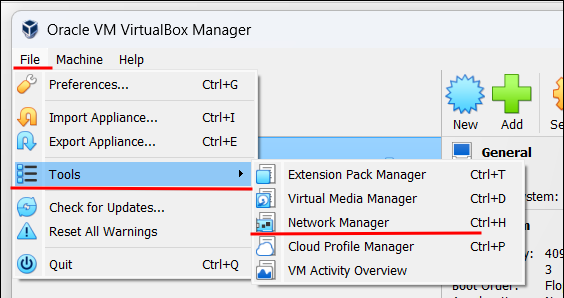
\includegraphics[width=0.5\textwidth]{./images/network-settings.png}
    \end{figure}
    \item Den Reiter \textit{Host-only Networks} auswählen.
    \item Mit \textit{Create} einen neuen Adapter erstellen.
    \item Die IPv4-Adresse muss auf 192.168.56.\textbf{1} konfiguriert sein damit die Virtuelle Maschine aufgefunden werden kann.
    \begin{figure}[!hbt]
        \centering
        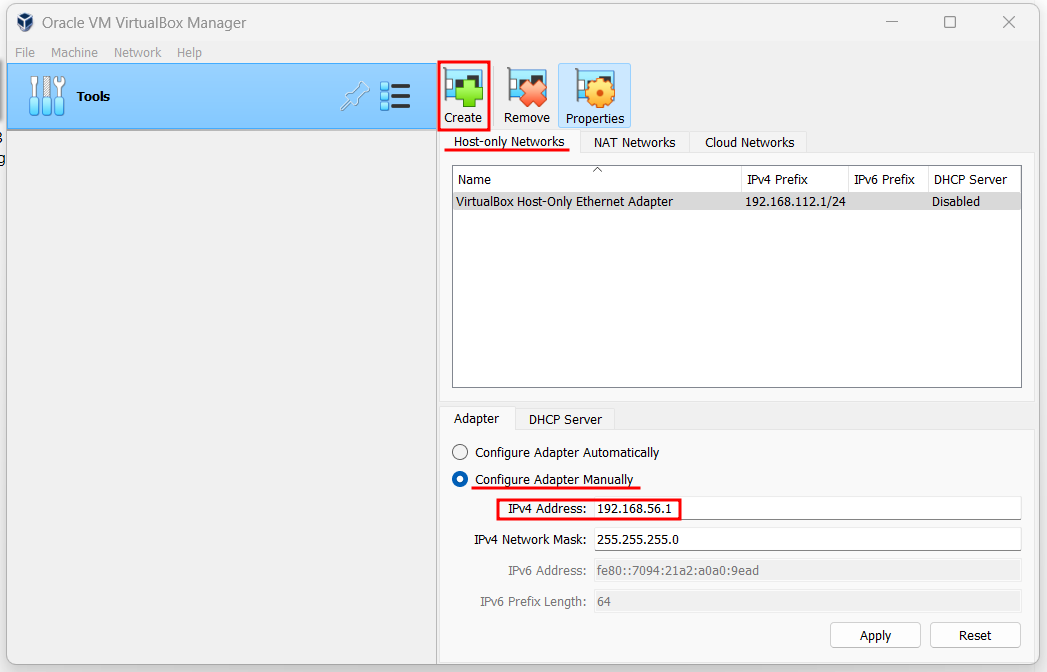
\includegraphics[width=0.9\textwidth]{./images/new-ho-network.png}
    \end{figure}
    \item Die Konfiguration der Laborumgebungs-VM aufrufen.
    \begin{figure}[!hbt]
        \centering
        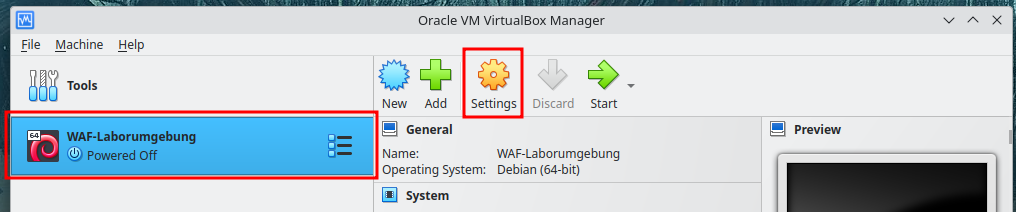
\includegraphics[width=0.9\textwidth]{./images/vm-settings.png}
    \end{figure}
    \item Den zweiten Netzwerk-Adapter unter (\textit{Network -> Adapter 2}) aktivieren.
    \item Den in Schritt 3 erstellten Adapter der VM zuordnen
    \begin{figure}[!hbt]
        \centering
        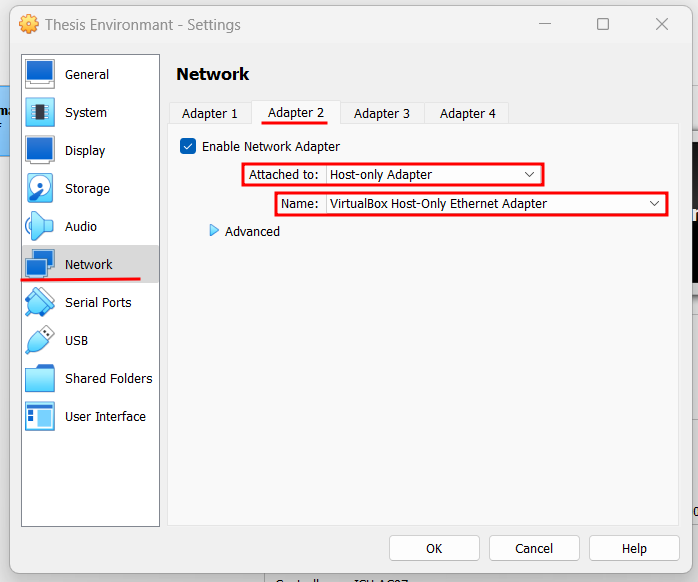
\includegraphics[width=0.9\textwidth]{./images/vm-ho-config.png}
    \end{figure}
\end{enumerate}
\pagebreak

Jetzt kann die Virtuelle Maschine gestartet werden.

\subsubsection{Websites aufrufen}
Die Lernumgebung bietet mehrerer Services mit denen interagiert werden kann, die alle mit Hilfe der Containervirtualisierungsumgebung Docker verwaltet werden.
Unter \href{https://192.168.56.2:9443}{\underline{https://192.168.56.2:9443}} steht eine Docker-Weboberfläche zur Verfügung, um die Bedienung zu erleichtern.
Die Login Daten sind:
\begin{itemize}
    \item \textbf{Username:} admin
    \item \textbf{Passwort:} waf-env12345
\end{itemize}

Nach einem Neustart der VM muss der WAF Docker-Container neu gestartet werden.
Auch wenn die WAF-Konfiguration geändert wurde, muss die WAF neugestartet werden damit die Änderungen übernomen werden.

Nach dem Login muss als erstes das lokale Environment und der Docker-Stack ausgewählt werden.
Dann kann die Laborumgebung (neu) gestartet werden:
\pagebreak

\begin{enumerate}
    \item \textit{Stacks -> waf-enf} auswählen
    \begin{figure}[!hbt]
        \centering
        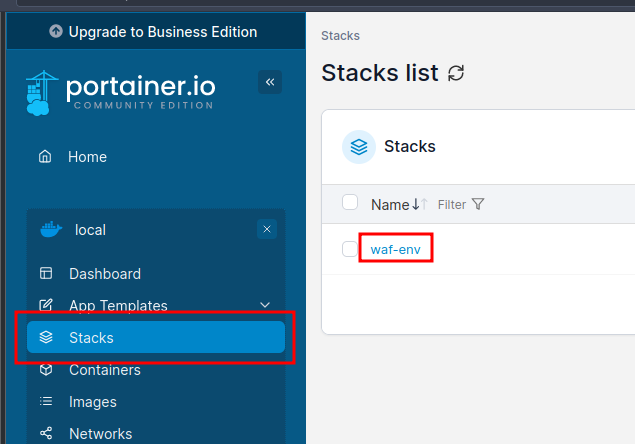
\includegraphics[width=0.9\textwidth]{./images/waf-env-porteiner.png}
    \end{figure}
    \item Hier können die Container ausgewählt und neugestartet werden
    \begin{figure}[!hbt]
        \centering
        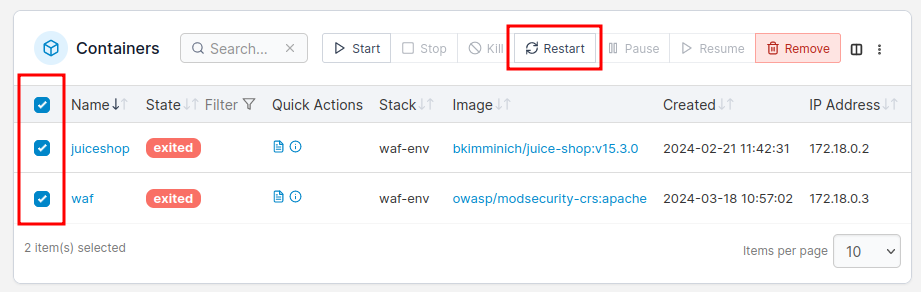
\includegraphics[width=\textwidth]{./images/restart-all.png}
    \end{figure}
\end{enumerate}

Nun sind alle Services der Laborumgebung aktiv und sind unter den folgenden URLs abrufbar:
\begin{enumerate}
    \item Verwundbare Anwendung mit WAF \href{https://192.168.56.2:443}{\underline{https://192.168.56.2:443}}
    \item Verwundbare Anwendung ohne WAF \href{http://192.168.56.2:3000}{\underline{http://192.168.56.2:3000}}
    \item Portainer \href{https://192.168.56.2:9443}{\underline{https://192.168.56.2:9443}}
\end{enumerate}

\subsubsection{Die WAF Konfigurationsdatei bearbeiten}

Der letzte Schritt zur Vorbereitung der Umgebung ist der Zugriff auf die WAF-Konfiguration.
Dies erfolgt über SSH auf die Virtuelle Maschine.
In dieser Anleitung wird die Verbindung mit der \textit{Visual Studio Code} Extension \href{https://marketplace.visualstudio.com/items?itemName=ms-vscode-remote.remote-ssh}{\underline{Remote - SSH}} erläutert.
Der Zugriff ist jedoch auch mit jedem anderen SSH-Client möglich.

\begin{itemize}
    \item \textbf{URL:} 192.168.56.2:22
    \item \textbf{Username:} waf-env
    \item \textbf{Passwort:} waf-env
\end{itemize}

Ist die Extension in vscode installiert, kann unter \textit{Remote Explorer -> SSH} mit dem \textit{+}-Icon eine neue Verbindung angelegt werden.

\begin{figure}[!hbt]
    \centering
    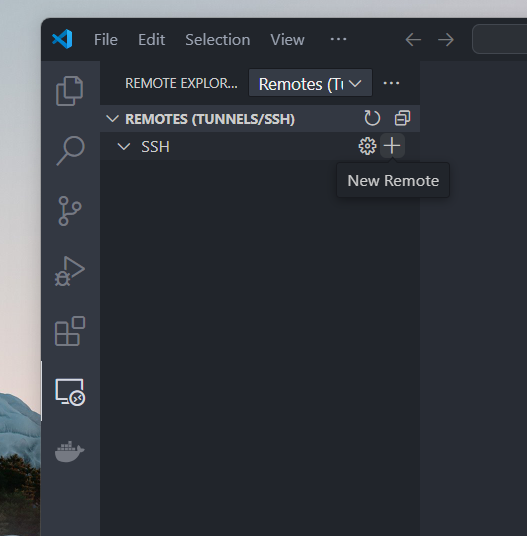
\includegraphics[width=0.5\textwidth]{./images/vscode-new-ssh.png}
\end{figure}

In dem sich öffnenden PopUp muss die SSH Verbindung eingetragen werden:

\textbf{waf-env@192.168.56.2}.

\begin{figure}[!hbt]
    \centering
    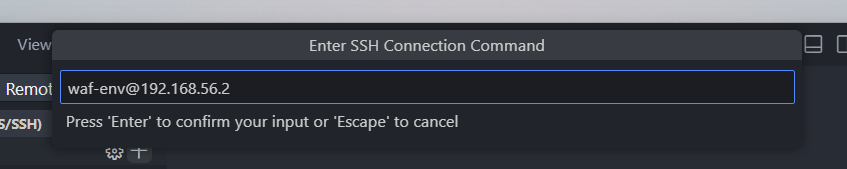
\includegraphics[width=0.9\textwidth]{./images/vscode-ssh-string.png}
\end{figure}

Es folgen PopUps in denen nach dem Gast Betriebssystem (Linux) und der Konfigurationsdatei für ssh gefragt werden.
Nutzen Sie die vorgeschlagenen Optionen.

Während dem Prozess wird wiederholt nach dem Passwort (\textit{waf-env}) gefragt.

Ist die Konfiguration abgeschlossen kann die Verbindung zu der VM mittels des Popups in der rechten unteren Ecke aufgebaut werden.

\begin{figure}[!hbt]
    \centering
    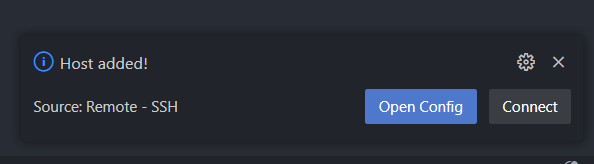
\includegraphics[width=0.7\textwidth]{./images/vscode-connect.png}
\end{figure}

Nachdem die Verbindung aufgebaut wurde muss zu dem Ordner navigiert werden, der die Konfigurationsdateien und Logs der WAF enthalten.

Im Reiter \textit{Explorer} kann der Ordner geöffnet werden.

\begin{figure}[!hbt]
    \centering
    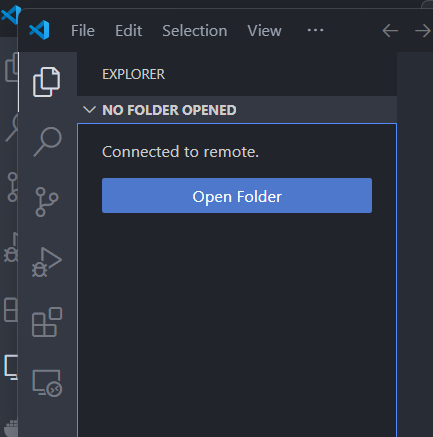
\includegraphics[width=0.7\textwidth]{./images/vscode-initiate-nw-dir.png}
\end{figure}

In dem PopUp den Pfad \textit{/home/waf-env/waf-env} angeben und bestätigen.

\begin{figure}[!hbt]
    \centering
    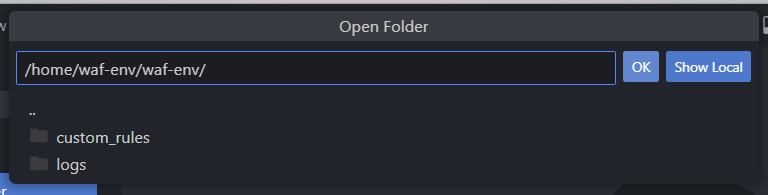
\includegraphics[width=0.7\textwidth]{./images/vscode-dir-path.png}
\end{figure}

Visual Studio Code merkt sich die Konfiguration die bei wiederholtem Aufruf im \textit{Remote Explorer} aufgerufen werden kann.

\subsection{Erste Konfiguration}

Die Ressourcen die Sie in der folgenden Liste finden, können Ihnen bei der Bearbeitung der Aufgabenstellungen behilflich sein.

\begin{itemize}
    \item Das \href{https://github.com/owasp-modsecurity/ModSecurity/wiki/Reference-Manual-(v3.x)}{\underline{ModSecurity Refernece Manual}} besonders die  \href{https://coreruleset.org/docs/rules/creating/}{\underline{Anleitung zum Schreiben von Regeln}}
    \item Auflistung der \href{https://pwning.owasp-juice.shop/companion-guide/latest/part2/README.html}{\underline{OWASP Juice Shop Challenges}}
    \item \href{https://github.com/refabr1k/owasp-juiceshop-solutions/tree/master}{\underline{Beispiellösungen}} für den Juice Shop
    \item Der Progress tracker des Juice Shops der unter der URL \textit{/\#/score-board} zu finden ist
\end{itemize}

\subsubsection{Sperren eines Pfades}
Um sich mit dem Aufbau einer ModSecurity Regel vertraut zu machen, soll der Zugang zu einem Pfad in der Website gesperrt werden.

In der Challenge \glqq\href{https://pwning.owasp-juice.shop/companion-guide/latest/part2/sensitive-data-exposure.html#_access_a_confidential_document}{\underline{access a confidential document}}\grqq\ ist der Zugriff auf ein Dokument möglich.

\textbf{Schreiben Sie eine neue Regel, die den Zugriff auf dieses Dokument verhindert und mit dem HTTP-Fehlercode 401 antwortet.}

\subsubsection{Parsen von HTTP Parameter}
In der Challenge \glqq\href{https://pwning.owasp-juice.shop/companion-guide/latest/part2/improper-input-validation.html#_give_a_devastating_zero_star_feedback_to_the_store}{\underline{give a devastating zero-star feedback to the store}}\grqq\ kann durch Bearbeiten eines HTTP-Requests ein Produkt mit 0 Sternen bewertet werden.

Vollziehen Sie das beschriebene Problem nach:
\begin{itemize}
    \item Was ist der Fehler, der die Schwachstelle ermöglicht?
    \item Welcher Parameter enthält die schadhaften Daten?
    \item Was wäre das korrekte Verhalten?
\end{itemize}

\textbf{Wenn Sie die Schwachstelle verstanden haben, schreiben Sie eine weitere Regel, die verhindert, dass ein Angreifer keine Daten außer den gültigen Werten an den Endpoint senden kann.}

\pagebreak

    \section{Aufgabenstellung Teil II}
    \label{sec:learning-unit-2}
    Sie haben sich im ersten Kapitel mit der Funktion der Laborumgebung vertraut gemacht und erste Regeln verfasst.
Dieses Kapitel befasst sich nun mit den ersten Angriffen die in ähnlicher Form auch an öffentlich erreichbaren Servern beobachtet werden können.
Im Folgenden werden Sie sich \textit{SQL-Injections} und \textit{Cross Site Scriptings (XSS)} genauer anschauen und WAF-Regeln für Angriffsszenarien im \textit{Juice Shop} schreiben, die diese in den Dort aufgeführten Fällen mittigieren.

\subsection{SQL Injections}
Die \href{https://portswigger.net/web-security/sql-injection/cheat-sheet}{SQL-Injection} ist eine sehr häufig auftretende Schwachstelle, die aus der unsauberen Weitergabe von Nutzerdaten an eine SQL Datenbank entstehen kann.

\subsubsection{SQL-Login-Bypass}
In der Challenge \glqq\href{https://pwning.owasp-juice.shop/companion-guide/latest/part2/injection.html#_log_in_with_the_administrators_user_account}{Log in with the administrator’s user account}\grqq\ kann die Passwort-Validierung bei einem Login umgangen werden.

Vollziehen Sie das beschriebene Problem nach:
\begin{itemize}
    \item Was muss in der Login Maske angegeben werden, um als administrator eingeloggt zu werden?
    \item Wie funktioniert der Login Prozess im Backend?
    \item Überlegen Sie sich Funktionierende Abwandlungen des Befehls zum Login als Administrator.
    \item Was haben diese Gemeinsam?
\end{itemize}

\textbf{Schreiben Sie eine WAF-Regel, die es ermöglicht den Angriff zu verhindern, indem Anfragen die den Login Bypass enthalten, abgelehnt werden.
Bedenken Sie, dass nicht nur ein Weg zu einer Ausnutzung führen kann.}

\subsubsection{SQL-Injections allgemein an drei Bespielen}

Der Juice Shop bietet weitere Möglichkeiten für SQL injections.
Zwei Beispiele sind die beiden Challenges \glqq\href{https://pwning.owasp-juice.shop/companion-guide/latest/part2/injection.html#_exfiltrate_the_entire_db_schema_definition_via_sql_injection}{\underline{database schema extraction}}\grqq\ und \glqq\href{https://pwning.owasp-juice.shop/companion-guide/latest/part2/injection.html#_log_in_with_benders_user_account}{log in with Bender’s user account}\grqq.

\begin{itemize}
    \item Welche SQL-Keywords werden in den Angriffen genutzt?
    \item Welche Mutationen dieser Keywords können verwendet werden und der Angriff funktioniert immer noch?
    \item Welche Probleme können Auftreten wenn die SQL-Keywords zu streng blockiert werden?
\end{itemize}

\textbf{Schreiben sie eine Regel die beide Angriffe aus den Challenges anhand der SQL Keywords verhindern kann. }

\subsection{Cross Site Scripting (XSS)}

Cross Site Scripting (XSS) ist eine weiter Klasse an Angriffen die in der aktuellen Cybersicherheit eine große Rolle Spielen.
Eine XSS-Schwachstelle zeichnet sich dadurch aus, dass Nutzereingaben die HTML, CSS oder JavaScript enthalten ausgeführt oder als Teil der Webseite dargestellt werden.

\subsubsection{Reflected XSS}

Die Challenge \glqq\href{https://pwning.owasp-juice.shop/companion-guide/latest/part2/xss.html#_perform_a_persisted_xss_attack_bypassing_a_server_side_security_mechanism}{Perform a persisted XSS attack bypassing a server-side security mechanism}\grqq\ enthält eine persistente XSS Schwachstelle.
Das heißt ein in HTML eingebetteter JavaScript Code-Abschnitt kann auf dem Server gespeichert werden und wird bei Aufruf auf einem Beliebigen client ausgeführt.

\begin{itemize}
    \item Was macht eine XSS-Schwachstelle aus?
    \item Können andere Elemente als \textit{iframes} und dem \textit{javascript:alert} genutzt werden?
\end{itemize}\

\textbf{Schreiben Sie eine Regel die das Ausnutzen der Schwachstelle verhindert.
Erweitern sie die Regel um eine Rewrite direktive, die den schadhaften Abschnitt aus der Anfrage entfernt sie aber an den Server weitergibt.}

\subsubsection{XSS Protection HTTP Headers}

Neben dem erkennen von XSS durch einen WAF existieren den HTTP-Header \textit{X-XSS-Protection} der in Browsern eie XSS-Schutzfunktion aktiviert.

\textbf{Schreiben Sie eine Regel die in allen Antworten des JuiceShops diesen Header setzt.}

\pagebreak

    %\section{Aufgabenstellung Teil II}
    %\pagebreak
\end{document}